\documentclass[../Main.tex]{subfiles}

\begin{document}
\chapter{Application Architecture}

\intro{

}

\defn{Software Architecture}{
    The fundamental organization of a system is embodied in its components, their relationships to each other, and to the environment, and the principles guiding its design and evolution.  (ISO/IEC/IEEE 42010, November 2011 )
}

There are many more definitions, but the one of the biggest
are:
\begin{enumerate}
    \item Bass, Clements and Kazman focuses on structure
    for example with architecture elements with their properties
    and relationships
    \item Jansen and Bosch empasizes design rational specifically
    desicion outcome and their justifications
    \item ISO/IEC/IEEE is a hybrid definition that combines elements from the other two
\end{enumerate}

Also Application Architecture as a sub-disiple of Software Architecture
that takes a logical viewpoint on end user apps and their architectures.
IT Architecture covers hardware and software and therefore is a superset.
(\href{https://arc42.org/overview}{ARC42 Software Architecture Templates}),
(\href{https://martinfowler.com/eaaCatalog/index.html}{Fowler's Enterprise Architecture}),
(\href{https://martinfowler.com/eaaDev/uiArchs.html}{Fowler's GUI Architectures})

Design challenges for the architecture of large and comples projects are divers and could contain:
\begin{itemize}
    \item User and channel diversity
    \item Process and resource integrity
    \item Integration need due to heterogeneity
    \item Complex data/domain models and processing rules
\end{itemize}

\section{Requirement Engineering}
\subsection{Architecural Significant Requirements}
All architecture is design, but not all design is architecture according to Grady Booch3; hence, it has to be de cided what is in and out of scope of any architectural activity. The notion of architectural significance has this purpose; it is a property of the requirements that are elicited/stated for a particular system and/or project, as well as design elements and decisions considered along the way. First and foremost, these requirements are non‑functional ones (also known as quality attributes); however, limiting architectural significance to these quality attributes is an oversimplification. Functional requirements can be architecturally significant as well, for instance if a feature request leads to the need for an additional external data provider that has to be inte grated via an Application Programming Interface (API).
\begin{enumerate}
    \item The requirement is directly associated with high business value or business risk
    \item The requirement is a concern of a particularly important stakeholder (for instance, the project sponsor or an external compliance auditor). 
    \item The requirement has runtime Quality-of-Service (QoS) characteristics (e.g., performance needs) that deviate from those already satisfied by the evolving architecture substantially.
    \item The requirement causes new or deals with one or more existing external dependencies that have unpredictable, unreliable and/or uncontrollable behavior. 
    \item The requirement has a cross-cutting nature and therefore affects multiple parts of the system and their interactions; it may even have system-wide impact. 
    \item The requirement has a first-of-a-kind character: e.g., the team has never built a component before that satisfies this particular requirement. 
    \item The requirement has been troublesome and caused critical situations, budget overruns or client dissatisfaction in a previous project in a similar context. 
\end{enumerate}

S. Toth asks the following five questions to classify the architectural significance of decisions that justify if and
how a requirement is met.
Just Enough Software Architecture:
\begin{enumerate}
    \item Is the decision hard to change later?
    \item Is the decision expensive to implement or execute?
    \item Are demanding, qualitative requirements stated?
    \item Are requirements difficult to map to existring solutions or experiences?
    \item Is the experience in the solution space weak?
\end{enumerate}

\subsection{NFR Catalogs and Taxonomies}

\defn{SMART}{
\begin{description}
    \item[Specific]  Targeting a particular area for improvement
    \item[Measurable] Quantifying, or at least suggesting, an indicator of progress
    \item[Assignable] Defining responsibility clearly
    \item[Realistic] Outlining attainable results with available resources. Time-related: Including a timeline for expected results 
\end{description}
The specific definitions of the words are not fixed.
}

The SMART criteria can be applied to NFR engineering.
\begin{itemize}
    \item Specific: Which feature or part of the system should satisfy the requirement?
    \item Measurable: How can testers and other stakeholders find out whether the requirement is met (or not)? Is the requirement quantified?
    \item A, R, T are requirements engineering and project management concerns: Useful interpretation in our NFR context: Agreed Upon, Realistic, Time-Bound
\end{itemize}

\defn{FURPS+}{
    Furps:
    \begin{itemize}
        \item Functionality
        \item Usability
        \item Reliability
        \item Performance
        \item Supportability
    \end{itemize}
    Furps+:
    \begin{itemize}
        \item Design constraints
        \item Implementation constraints
        \item Physical constrains
        \item Interface contraints
    \end{itemize}
}
\newpage
\subsection{Quality Attribute Scenario (QAS)}
Quality attributes describe how a system provides its functionality, not how.

\begin{figure}[H] 
    \centering
    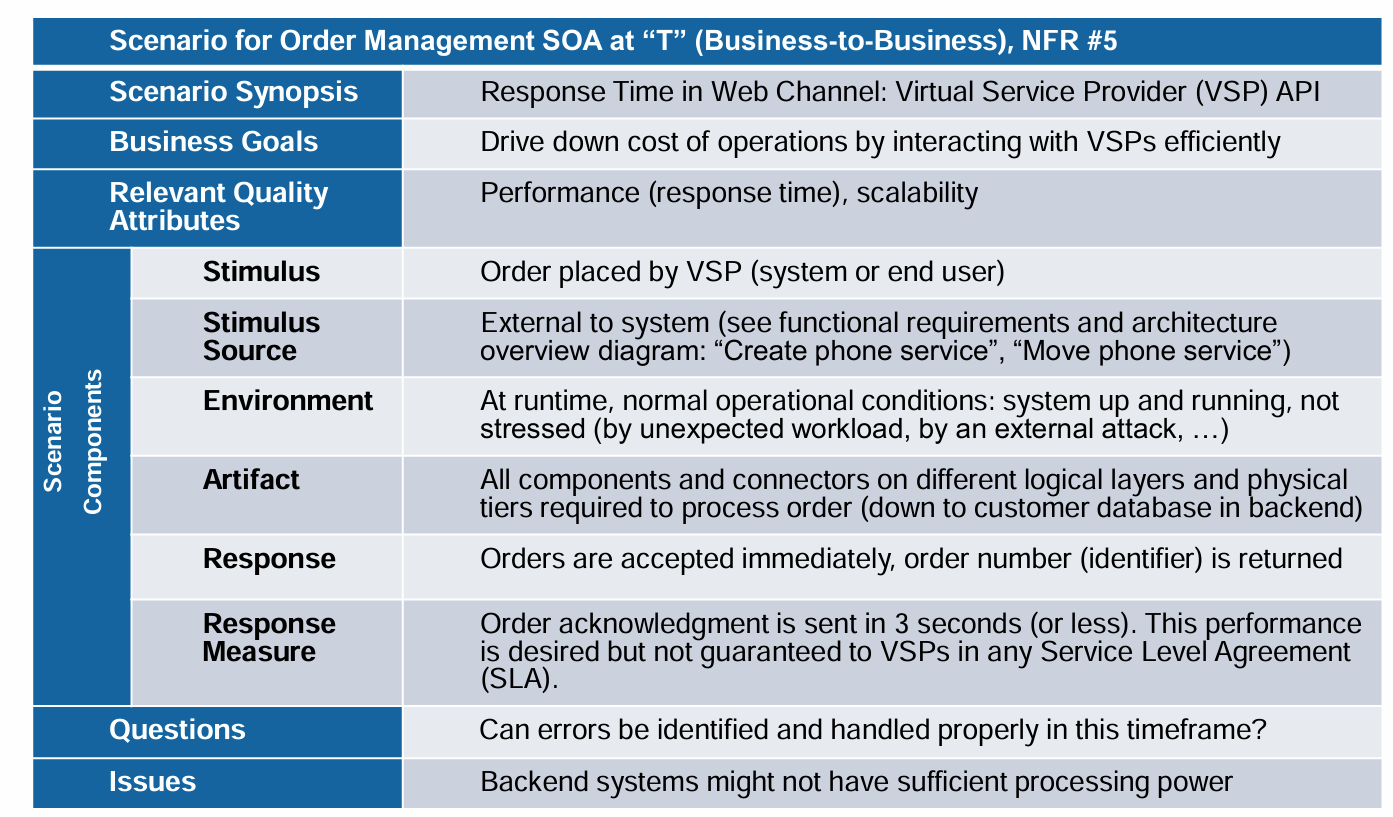
\includegraphics[width=1\linewidth]{Images/qas.png}
    \caption{QAS}
    \label{fig:qas}
\end{figure}

\subsection{Landing Zones}
Rather than establishing one measurable target define three.
This helps agree upon a range rather than one single value.
This is similar to release criteria but allows for tolerances
in acceptable values. Moreover it allows for some flexibility
in meeting goals.

\begin{figure}[H]
    \centering
    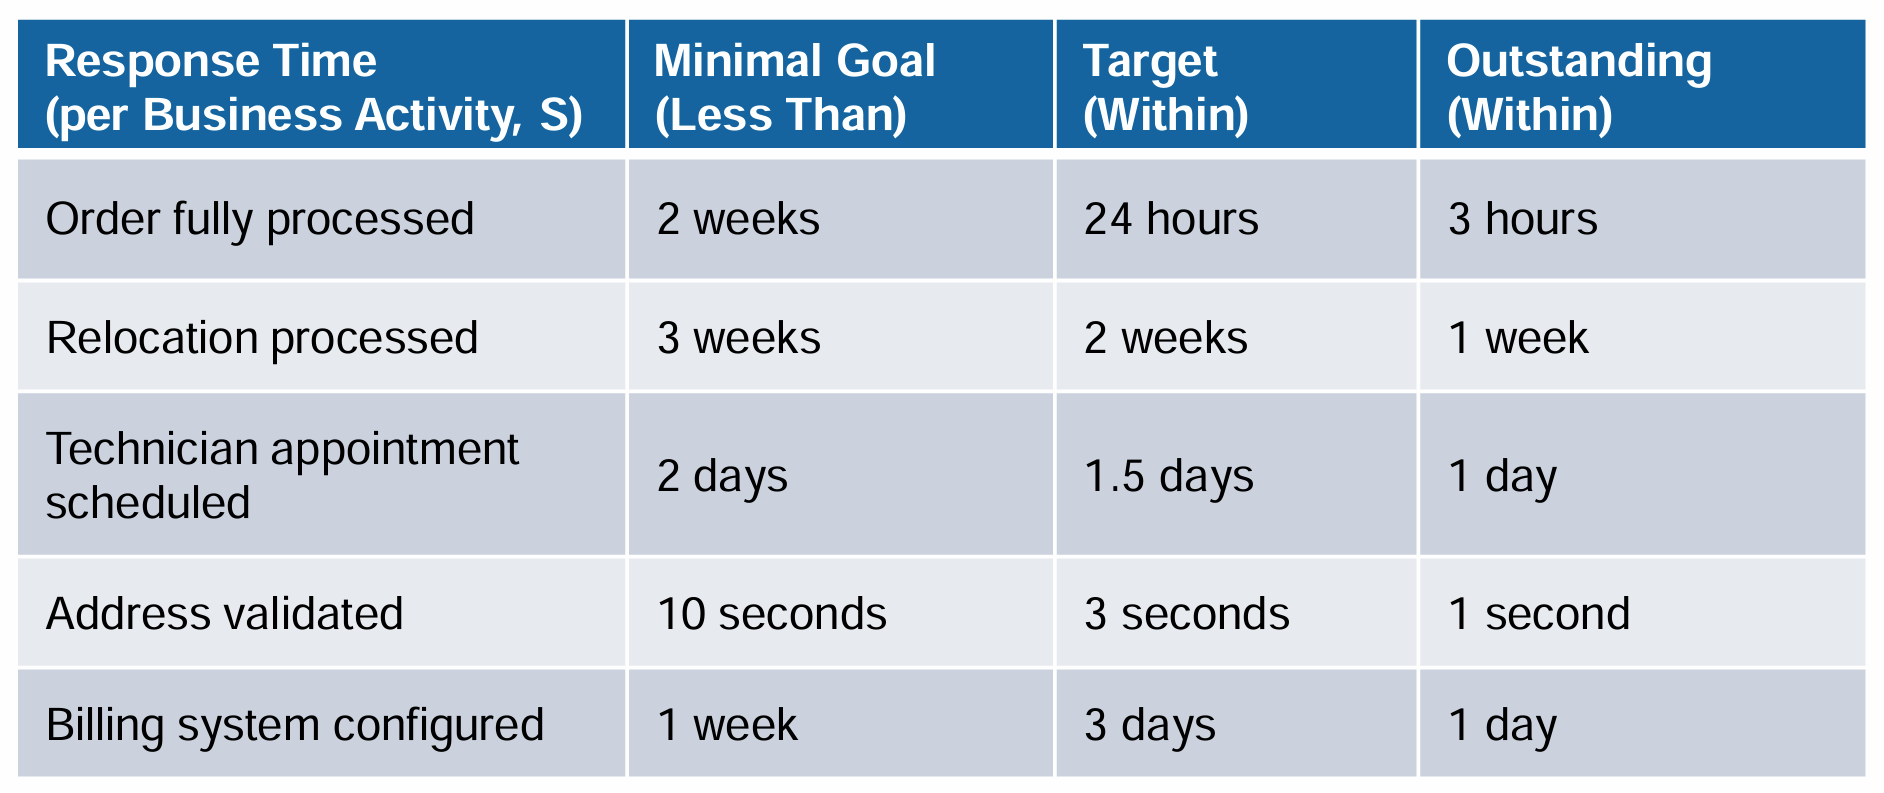
\includegraphics[width=1\linewidth]{Images/landingzone.png}
    \caption{Landing Zones}
\end{figure}

\subsection{Quality Utility Trees}
Quality Utility Trees (QUT) can be used to refine
each toplevel taxonomy topic. In the trees the leaves
represent QAS prioritized by value and risk.

\begin{figure}[H]
    \centering
    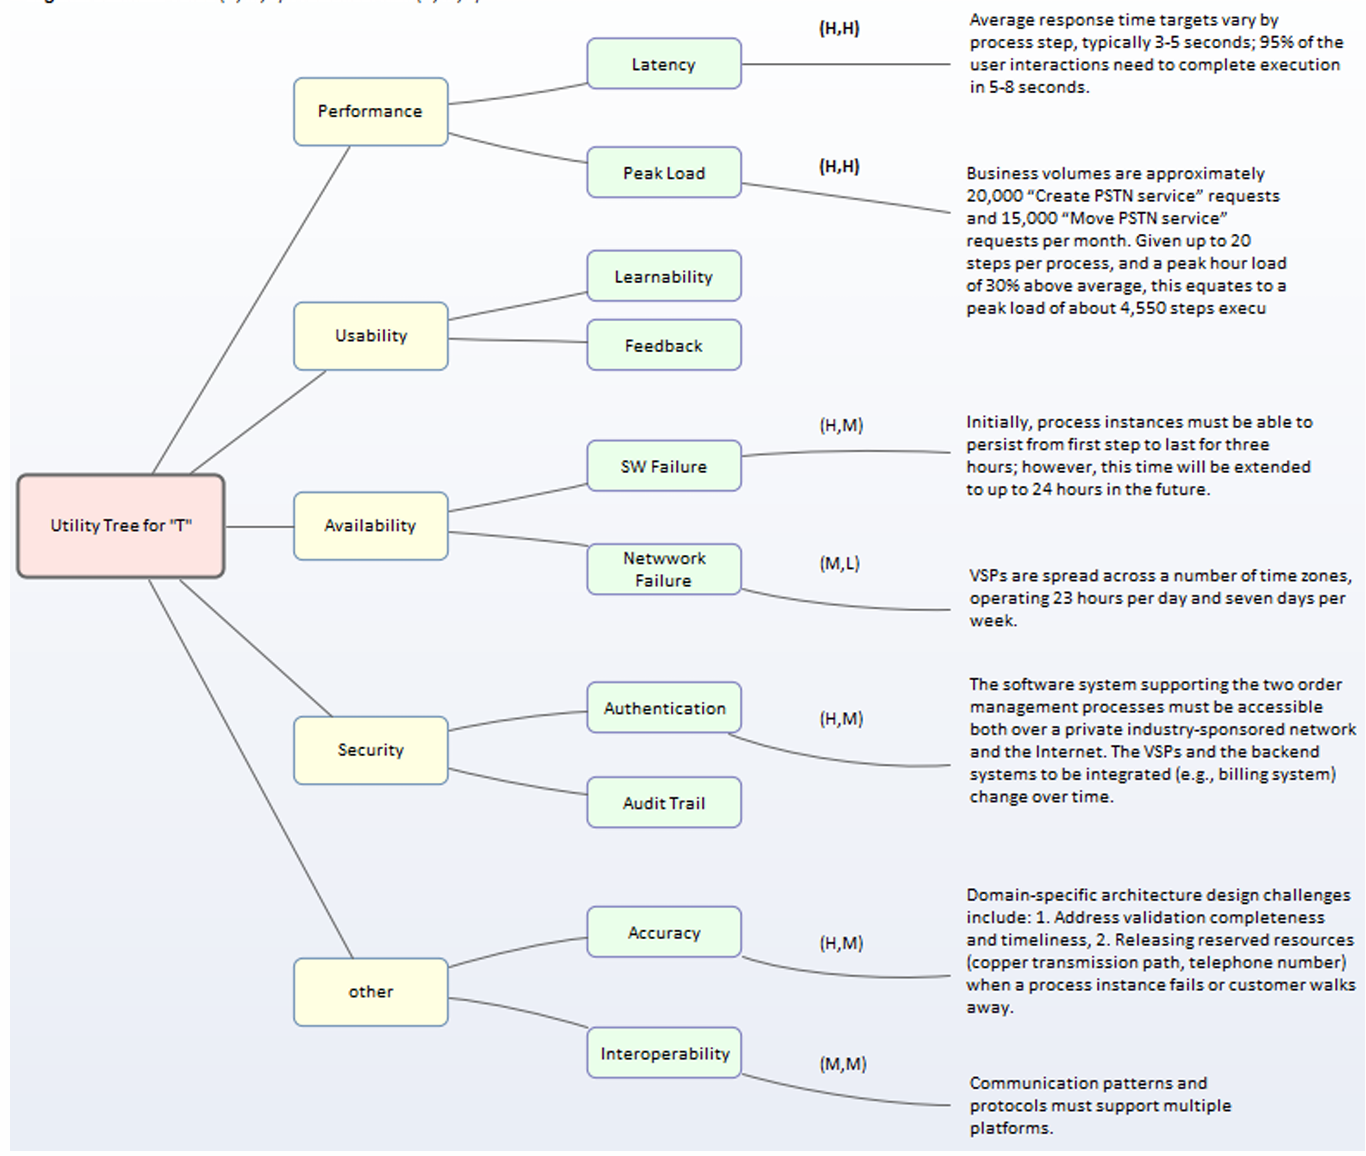
\includegraphics[width=0.5\linewidth]{quality-utility-trees.png}
    \caption{Quality Utility Trees}
\end{figure}

\subsection{System Context Diagrams}
SCD should be use to identify external dependencies.
In this method we represent systems as block boxes and
depict interactions with external entities.
It can identity the information and control flow.

\begin{figure}[H]
    \centering
    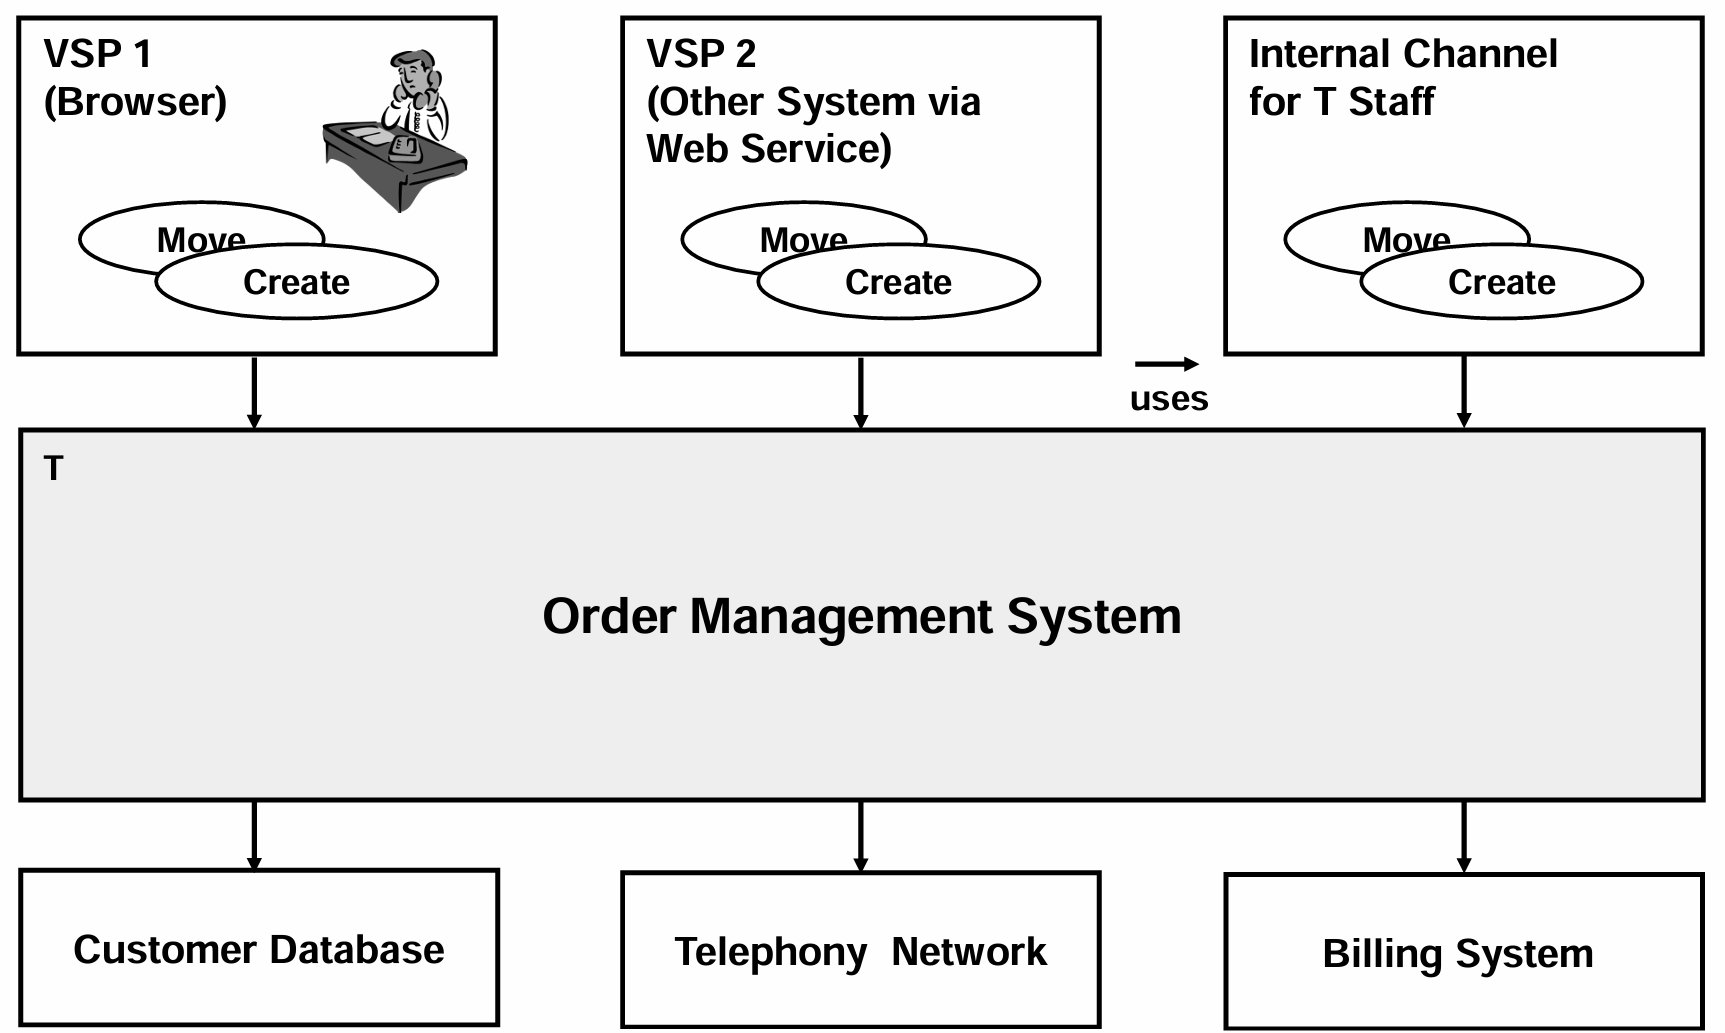
\includegraphics[width=0.5\linewidth]{system-context-example.png}
    \caption{System Context Diagram Example}
\end{figure}

%\subsection{Twin Peaks}
% Analysis and synthesis do not follow each other in a waterfall
% Cross fertilization, you learn as you go: “Twin Peaks” Model
%\begin{figure}[H]
%    \centering
%    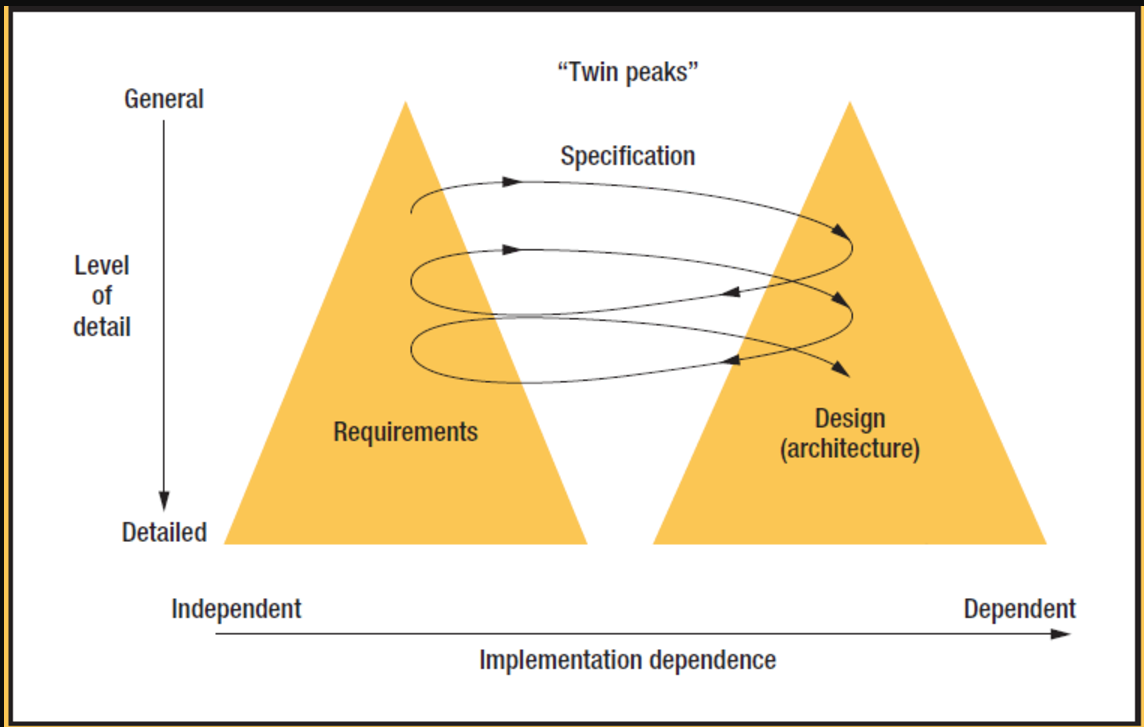
\includegraphics{Images/twinpeak.png}
%    \caption{Twin Peak Design}
%    \label{fig:twinpeakdesign}
%\end{figure}
\newpage

\section{Solution Strategy}
The term Solution Strategy is from Gernat Starke (arc42).
It corresponds to the Inception and Elaboration phases in
RUP. It includes the big decisions
one should make to which would later be costly to change (Grady Booch).
IBM defines some reference goals for the solution stategy:
\begin{itemize}
    \item Provide a single place to find important decisions
    \item Make explicit the rationale and justification
    \item Preserve design integrity
    \item Ensure that architecture is extensible and evolving
    \item Provide a reference of documented decisions
    \item Aboid unnecessary reconsideration of the same issues
\end{itemize}

\defn{Solution Strategy (arc42)}{
Are fundamental decisions and solution strategies,
that shape the system's architecture. These include:
\begin{itemize}
    \item Technology decisions
    \item Decisions about the top-level decomposition of the system, e.g. usage of an architectural pattern or design pattern
    \item Decisions on how to achieve key quality goals
    \item Relevant organizational decisions, e.g. selecting a development process or delegating certain tasks to third parties.
\end{itemize}
 \href{https://docs.arc42.org/section-4/}{ARC42 SS Template}
}

\subsection{Y-Template}
The Y-Template can be used to make decisions more
descriptive. It links AD to design context and NFRs
and shows tradeoffs between qualities.

\begin{figure}[H]
    \centering
    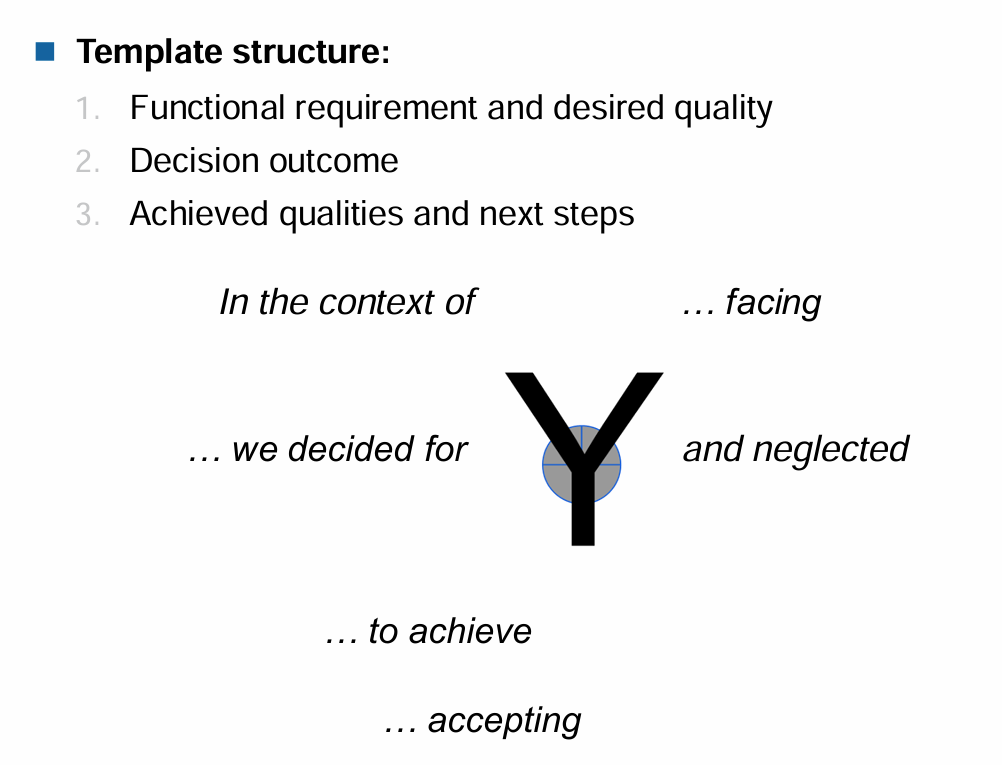
\includegraphics{Images/yarchitecturedesign.png}
    \caption{Y-Template for Architecture Design Decision}
\end{figure}

%\subsection{Architectural Decision Records}
%\href{https://adr.github.io/}{ADR Templates}

\subsection{Logical Layering and Tiers}

\begin{figure}[H]
    \centering
    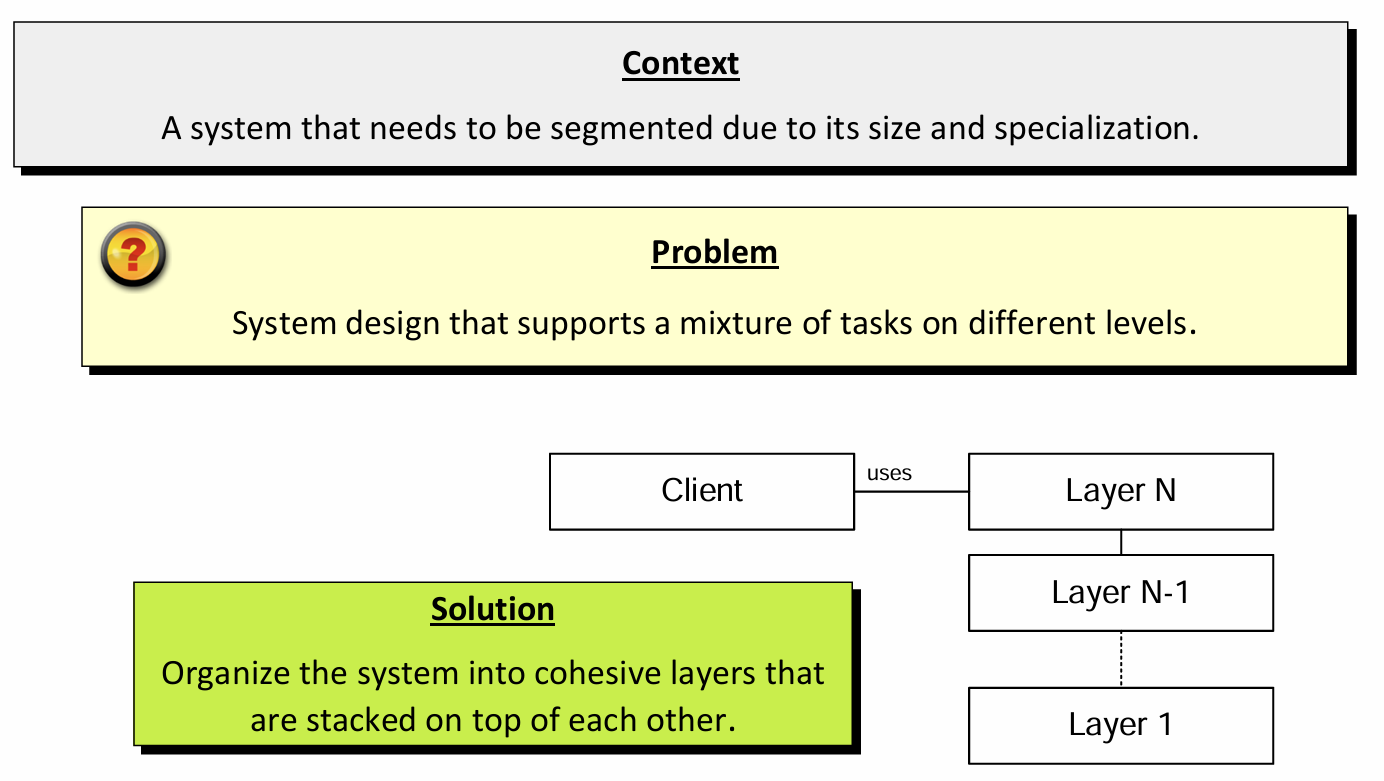
\includegraphics[width=1\linewidth]{Images/logicallayering.png}
    \caption{Logical Layering}
\end{figure}

The definition of layers and tiers is a typical
big decision in solution strategy:
\begin{itemize}
    \item In the logical and implementation view
    layers separate concerns
    \item In the process and physical view
    tiers distribute the workload
\end{itemize}

\defn{Layers}{
    Layers describe the logical groupings 
    of the functionality and components in an application.
}

\defn{Tiers}{
    Tiers describe the physical distribution of the 
    functionality and components on separate servers, 
    computers, networks, or remote locations.
}

Although both layers and tiers use the same set of names 
(presentation, business, services, and data), 
remember that only tiers imply a physical separation.
It is quite common to locate more than one layer on the
same physical machine (the same tier). You can think of
the term tier as referring to physical distribution
patterns such as two-tier, three-tier, and n-tier.
The following architectural drivers and decision making criteria (or forces in pattern terminology) apply:
\begin{itemize}
    \item Businessneedsvs.construction complexity
    \item Processing style: online (transactional) vs. offline (batch processing)
    \item Distribution vs. performance, security, consistency
    \item Softwaredistribution cost
    \item Reusability vs. performance vs. complexity
    \item Supportability
\end{itemize}

\subsubsection{Typical Layering}
An often used logical layering scheme is:
\begin{itemize}
    \item Presentation Layer
    \item Business Logic Layer
    \item Data Access Layer
\end{itemize}
Its most popular in enterprise application development but also
applicable in other genres.
The layer pattern itself does not imply process/server boundary and any use of remoting is optional.


%\begin{description}
%\item[Presentation Layer:] End users and external systems only talk to presentation layer. Rationale: isolation from backend. Presentation layer talks to business logic. Rationale: support multiple presentations of same logic
%\item[Business Logic:] Business logic uses data access layer to communicate with database and backend systems. Which can be swapped in and out
%\end{description}

\begin{figure}[H]
    \centering
    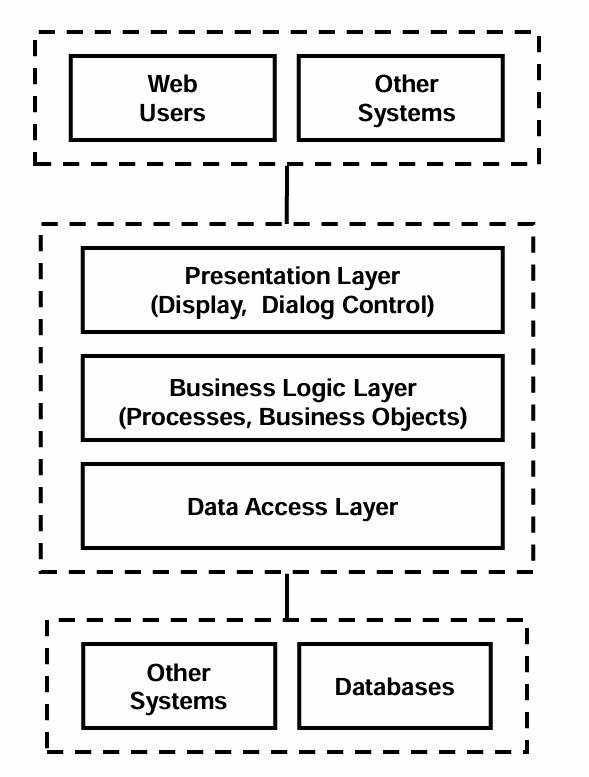
\includegraphics[width=0.5\linewidth]{Images/logicallayer.png}
    \caption{Logical Layers}
\end{figure}

With many options how to assign layers to tiers: Layer boundary or
within layer,  Single or multiple assignments.

\subsubsection{Client Server Cuts (CSC)}
The five CSCs have been captured as distribution patterns 
rather early in the evolution of object‑oriented pro gramming
and integrated business information systems (Renzel and Keller (1997)).
\begin{figure}[H]
    \centering
    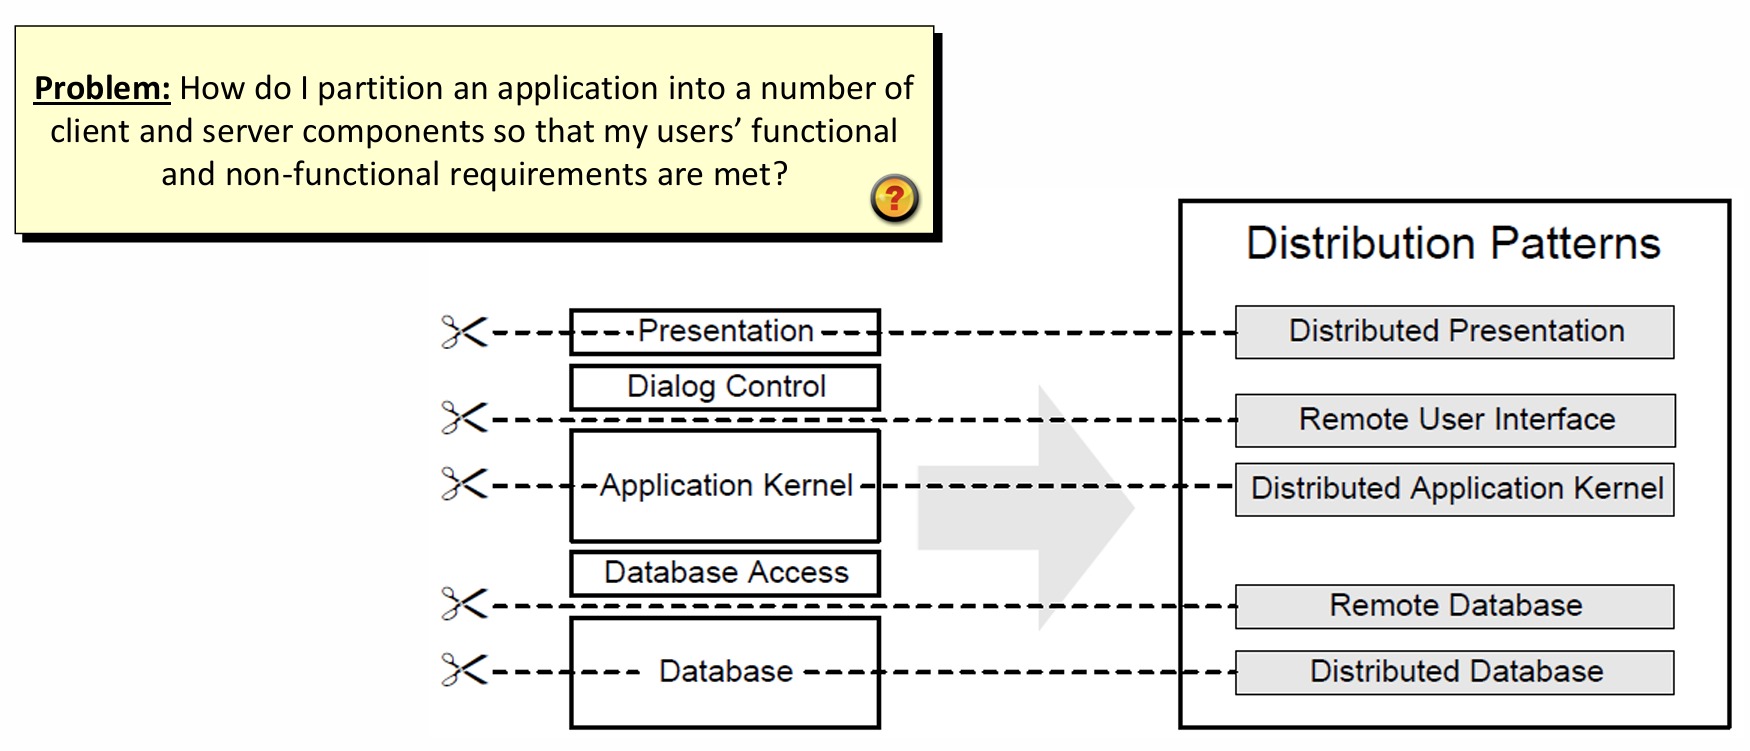
\includegraphics[width=1\linewidth]{Images/csc.png}
    \caption{CSC}
\end{figure}

\begin{figure}[H]
    \centering
    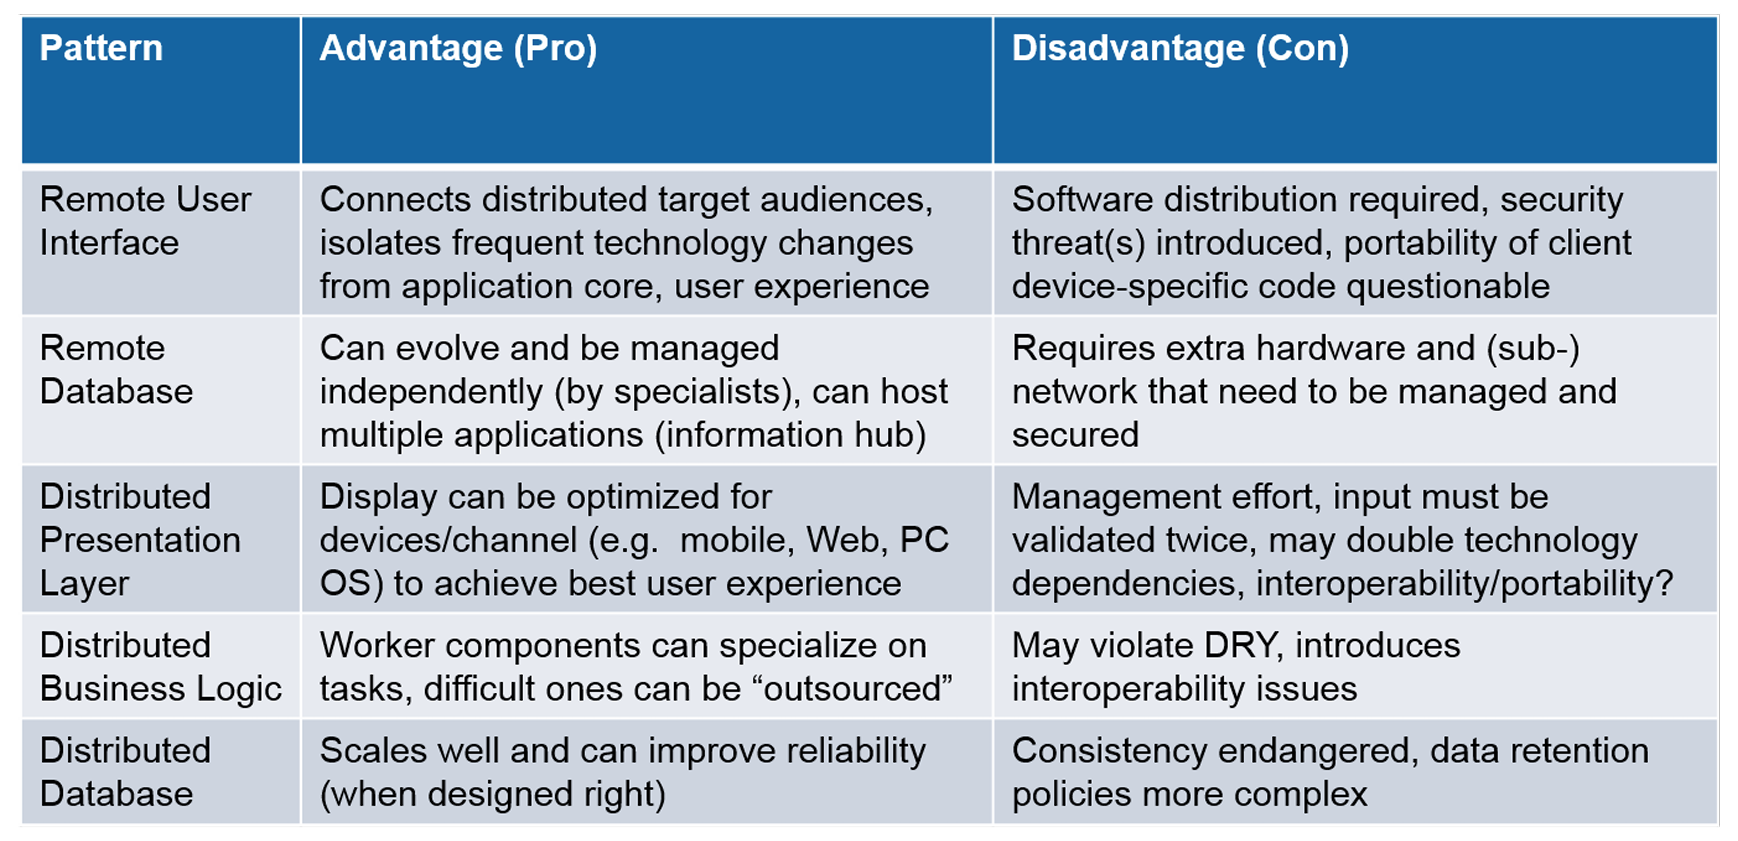
\includegraphics[width=1\linewidth]{Images/csc-pro-con.png}
    \caption{CSC Pro and Cons}
\end{figure}

\subsection{Big Architectural Decisions}
\begin{enumerate}
    \item Those with high arch. significance score
    \item Those requiring financial investment; those with tough consequences
    \item Those that take a long time to execute upon
    \item Those with many or still unclear outgoing dependencies
    \item Those that take a long time to make according to DoD (ecADR)
    \item Those with a high level of abstraction 
    \item Those with problem/solution space outside of team's comfort zone 
\end{enumerate}
\href{https://github.com/adr/madr}{MADR Templates}

\subsection{Container}
Container are application-level frameworks for tier 2 of a 2-tier or 3-tier
application. Application level containers are not to be confused with container-based
applications on the os system level. 

In the C4 model, a container represents an application or a data store.
    A container is something that needs to be running in order for the overall software system to work.

A container is essentially a runtime boundary around some code that is
being executed or some data that is being stored. The name “container”
was chosen because I wanted a name that didn’t imply anything about the
physical nature of how that container is executed. For example,
a single Java EE server like Apache Tomcat can run multiple web
applications inside a single Java Virtual Machine, although each of
those web applications is essentially isolated from the others.
At development time I might have three web applications running on
a single Apache Tomcat server, while each web application may be
deployed onto a dedicated Apache Tomcat server in a live environment.
In this situation, each web application is a “C4 container”,
with the deployment being a seperate concern.

\subsection{Container Architecture Patterns}
\paragraph{Inversion of Control (IoC)}
IoC enables (container) frameworks to control server-side execution
and achieve extensibility with custom components even without recompilation.
With this pattern a framework (or software component) has control and
manages the application component instances.
The components know the interfaces of their members.
External requests arrive at the framework which redispatches them.

The overall goal is to enable high configuration flexibility
which leads to beeing able to swap implementations in and out which
is good for:
\begin{itemize}
    \item DevOps automation, CI/CD
    \item Running parallel versions
    \item Mocking
    \item Cloud vs inhouse deployment
\end{itemize}

\begin{figure}[H]
    \centering
    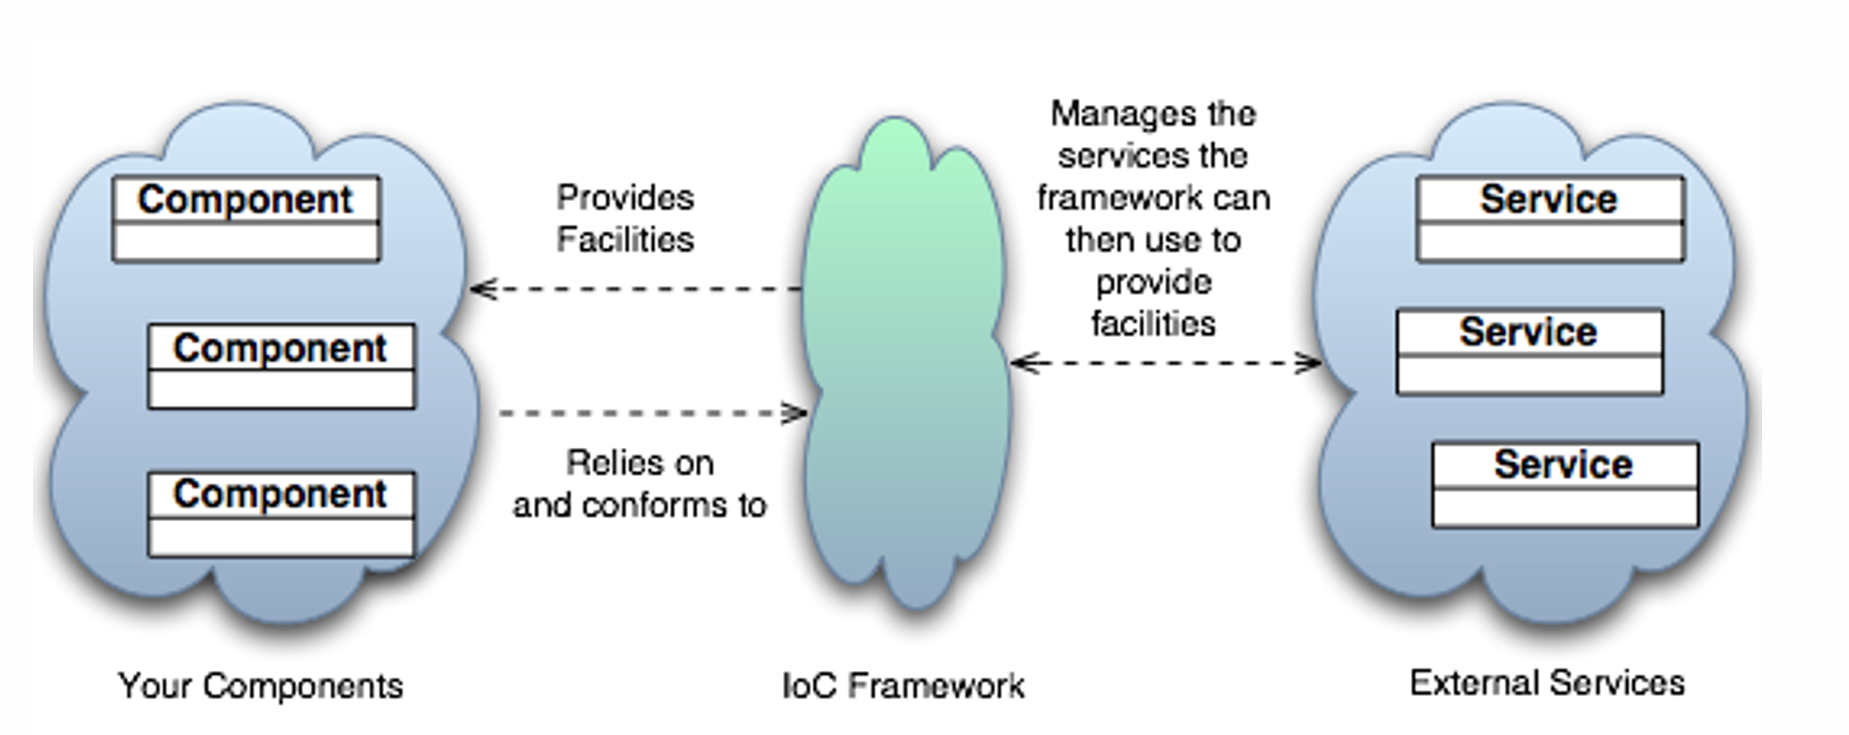
\includegraphics[width=1\linewidth]{Images/ioc.png}
    \caption{Inversion of Control}
\end{figure}

Interface implementations are received using dependency injections.
Which is a pattern that gives an object its instance variables.
This is good for isolating classes during testing and for systems
with many configurations. It is a one-step class member initialization.

\begin{figure}[H]
    \centering
    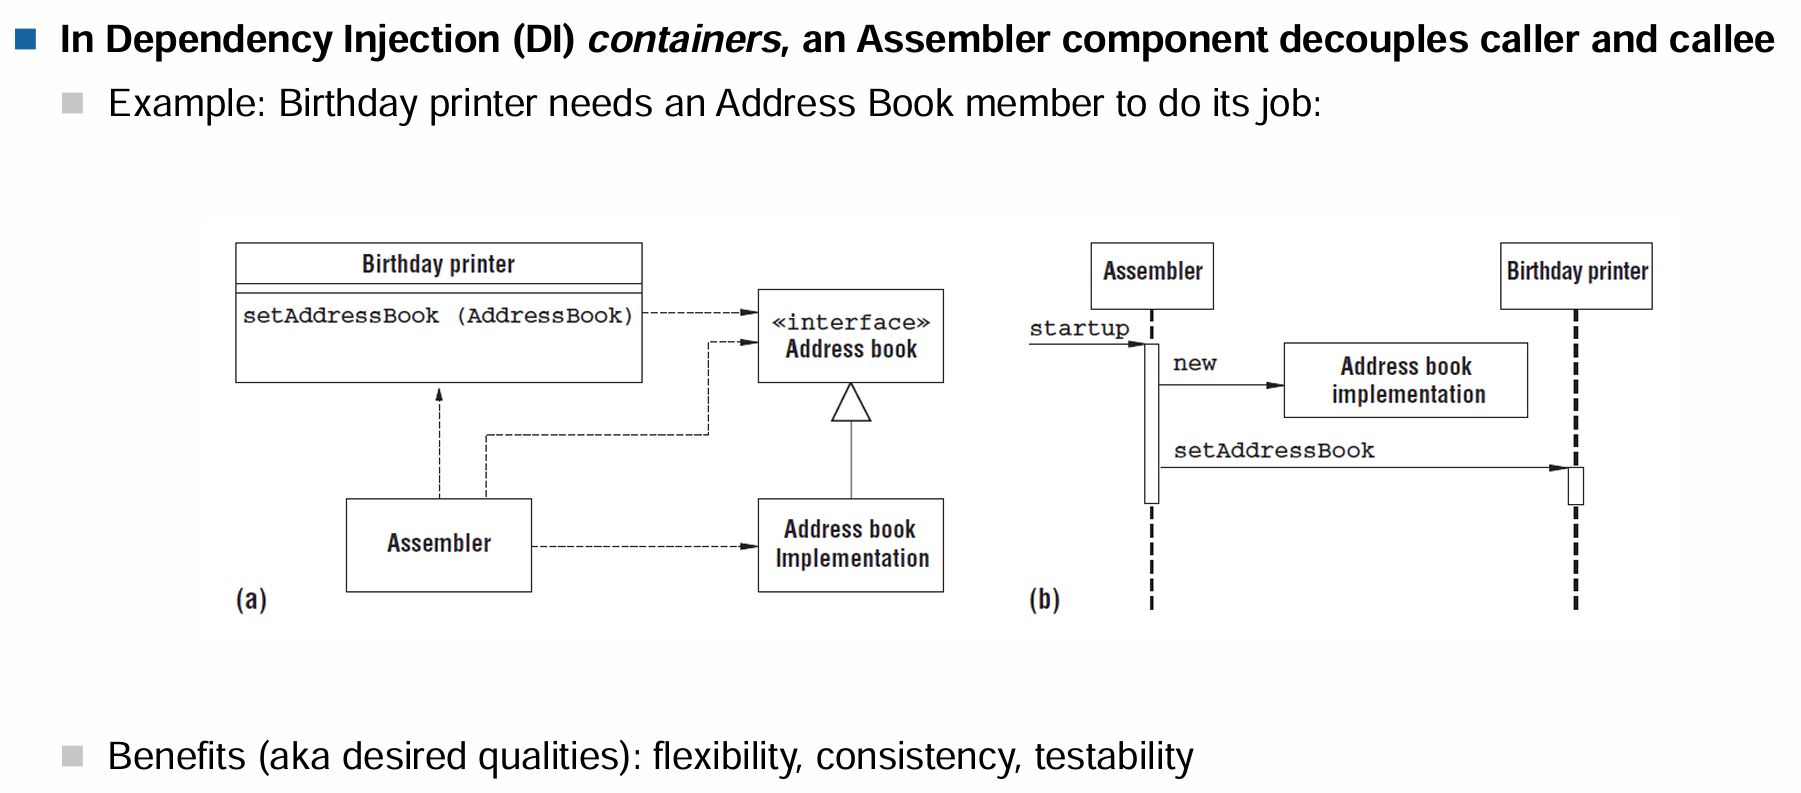
\includegraphics[width=1\linewidth]{Images/dep-injection.png}
    \caption{Dependency Injection}
\end{figure}

\subsubsection{Server-Side Container Architecture (Spring Boot)}

\begin{figure}[H]
    \centering
    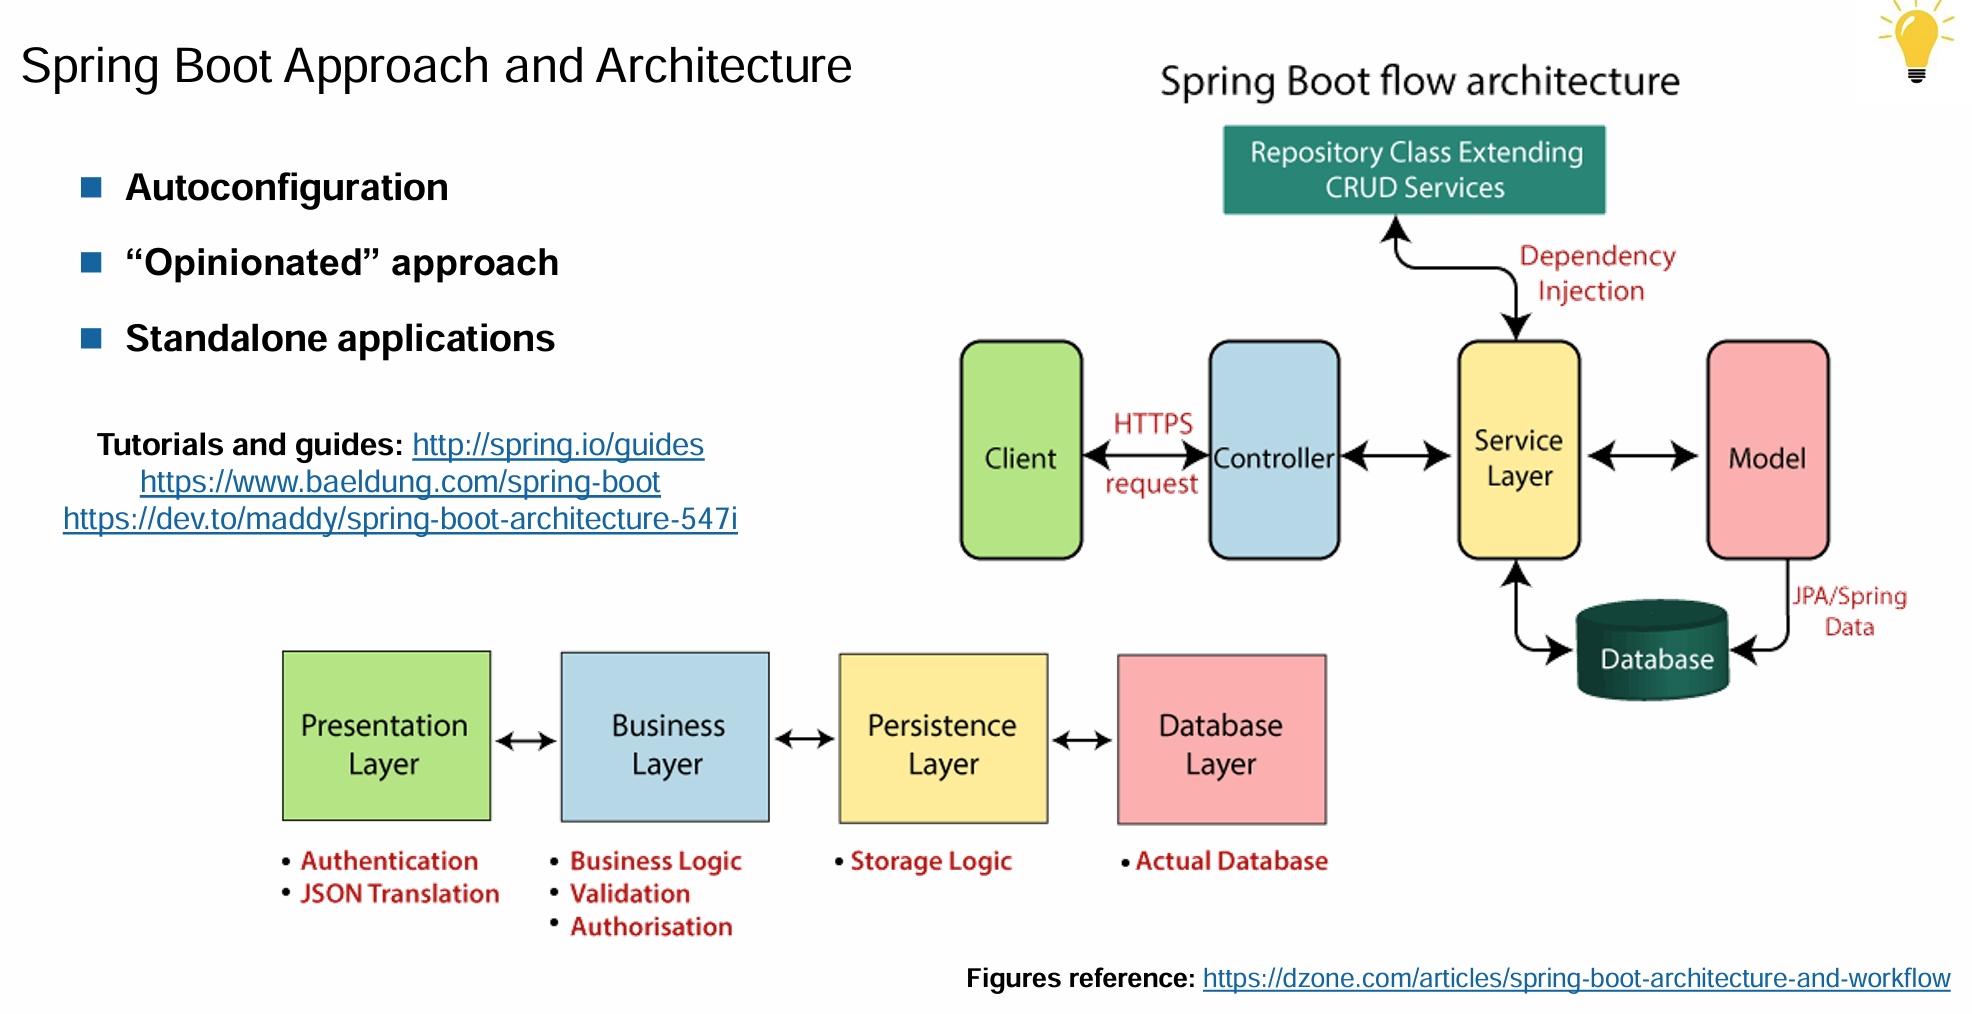
\includegraphics[width=1\linewidth]{Images/spring-boot-arch.png}
    \caption{Spring Boots Architecture Overview}
\end{figure}

\begin{figure}[H]
    \centering
    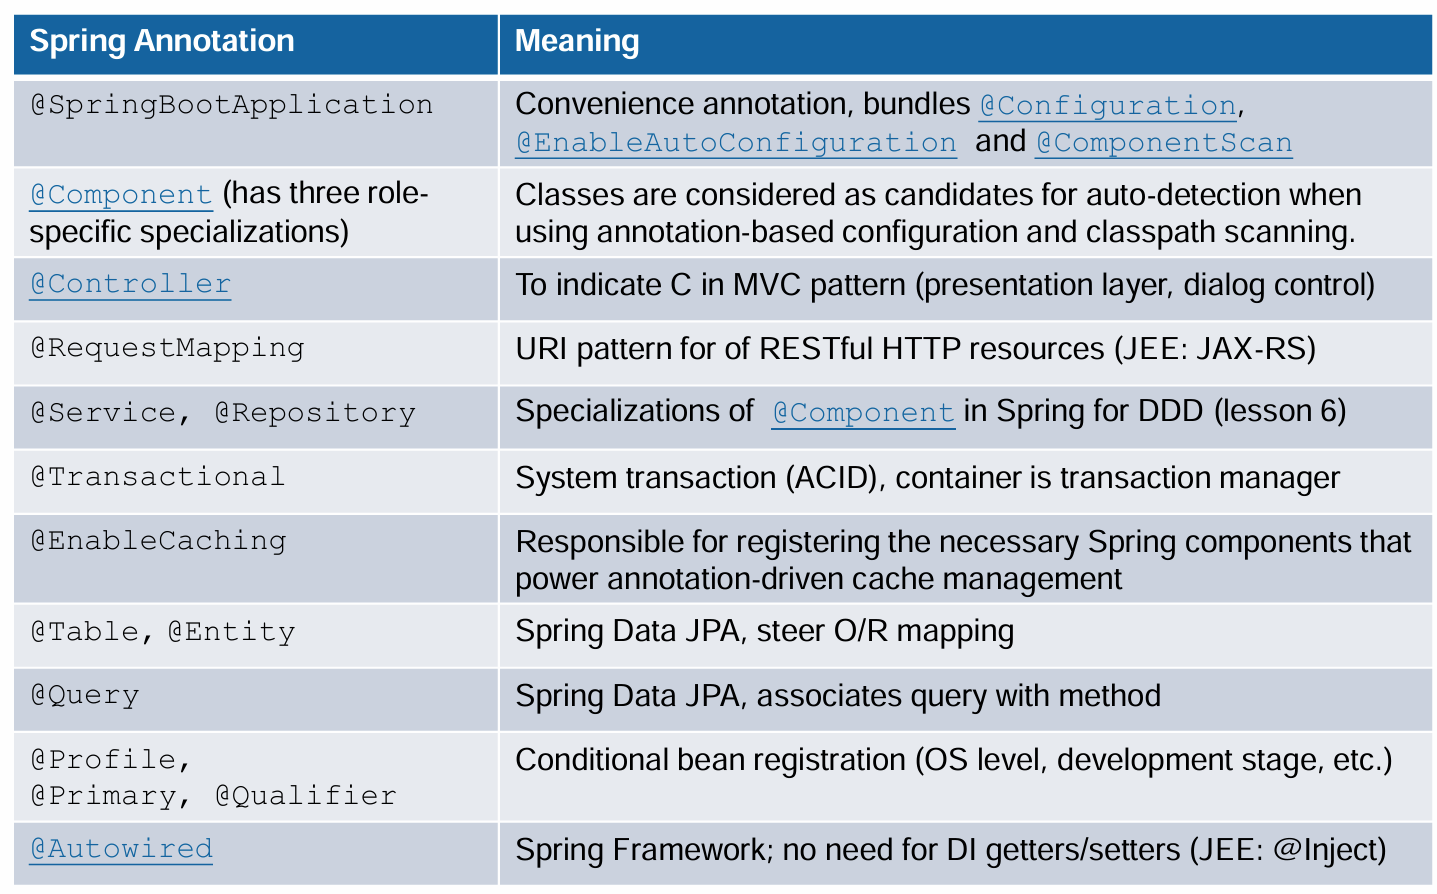
\includegraphics[width=1\linewidth]{Images/spring-boot-annotations.png}
    \caption{Key Spring Annotations}
\end{figure}

\subsection{Components}
A component is a grouping of related functionality encapsulated behind a
well-defined interface. If you're using a language like Java or C\#,
the simplest way to think of a component is that it's a collection of
implementation classes behind an interface.

With the C4 model, components are not separately deployable units.
Instead, it's the container that's the deployable unit. In other words,
all components inside a container execute in the same process space.
Aspects such as how components are packaged (e.g. one component vs
many components per JAR file, DLL, shared library, etc) is an
orthogonal concern.

The components that we deal with in solution strategy are candidate components.
A candidate component is anintermediate/preliminary architectural element
used for planning, decision making, architectural prototyp ing.
The candidate components are subject to continuous refinement and
consolidation efforts (architectural refactoring).

\begin{figure}[H]
    \centering
    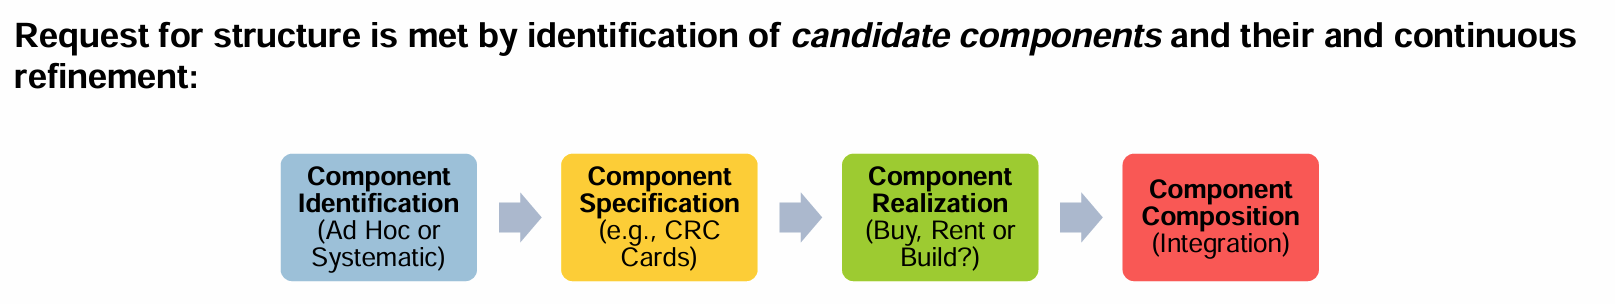
\includegraphics[width=1\linewidth]{Images/candidatecomponents.png}
    \caption{Candidate Components}
\end{figure}
\newpage

\subsection{Component Interactions}
When modeling NFR with FURPS many design issues that also
concern dynamcs are yielded. Hence, architecture is not only
about structure, but also behaviour.
You should understand how (instances of) building blocks of
your system perform their job and communicate at runtime.
You will mainly capture scenarios in your documentation
to communicate your architecture to stakeholders that are
less willing or able to read and understand the static models
(building block view, deployment view). (\href{http://docs.arc42.org/section-6/}{arch42})

\begin{figure}[H]
    \centering
    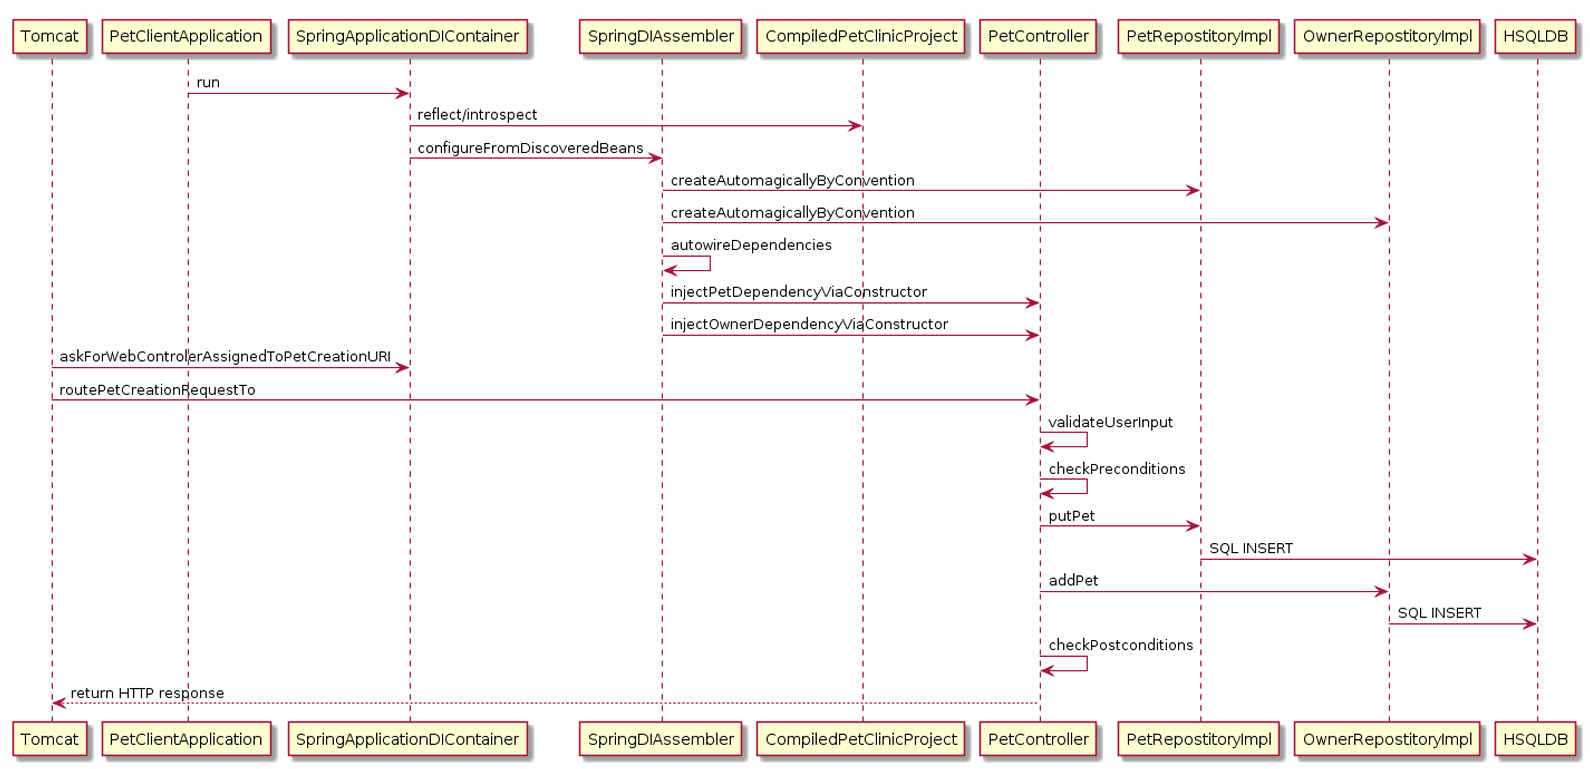
\includegraphics[width=1\linewidth]{Images/component-dynamics.png}
    \caption{Component Dynamics Example}
\end{figure}

\subsection{Common Components}
\begin{figure}[H]
    \centering
    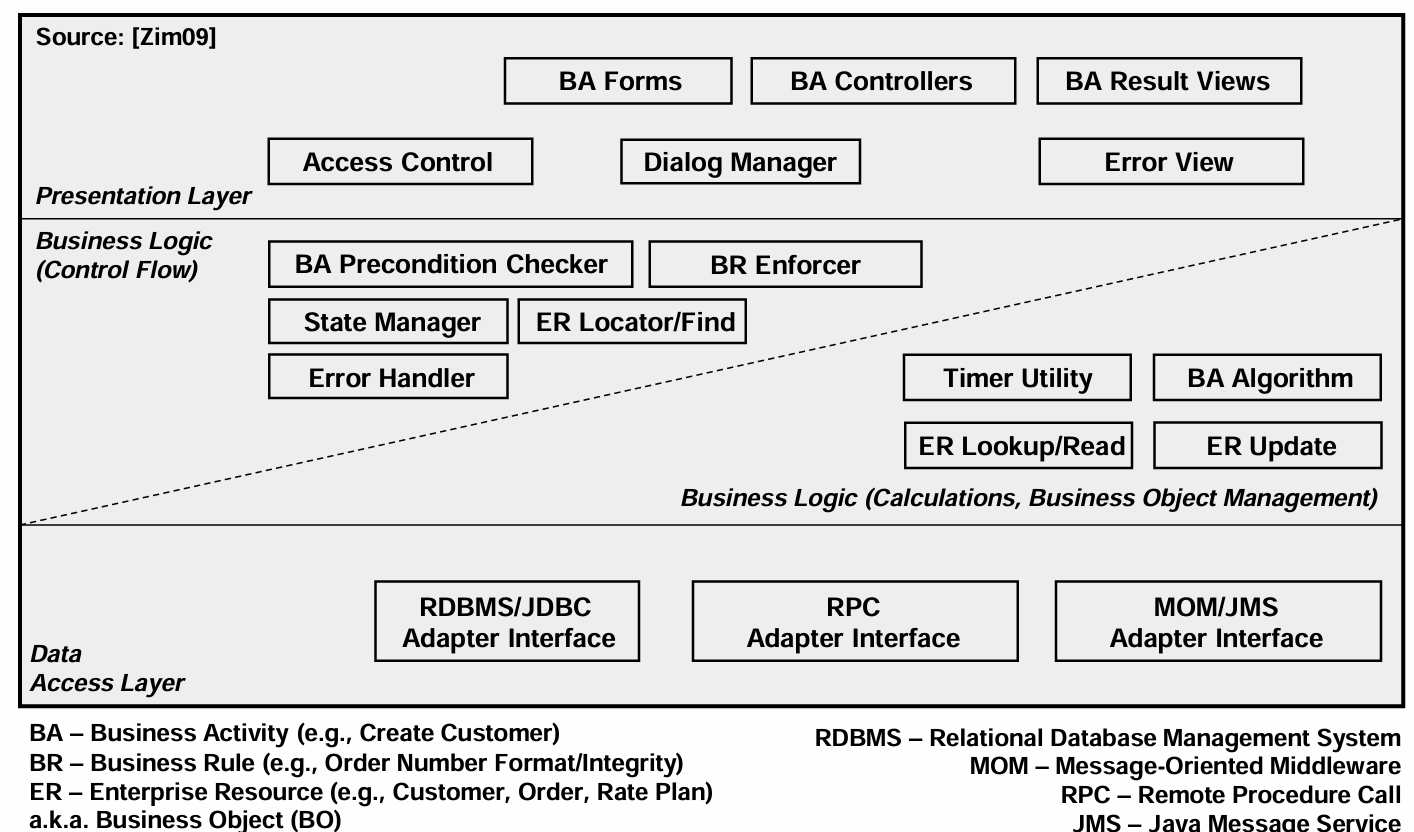
\includegraphics[width=1\linewidth]{Images/commoncomponents.png}
    \caption{Common Components}
\end{figure}

\subsection{Component Modeling}
A candidate component is an architectural element in the logical 
viewpoint grouping related responsibilities that jointly satisfy
one or more (non-)functional requirements so that design and
implementation work can be planned and component realization
decisions can be made.

\begin{figure}[H]
    \centering
    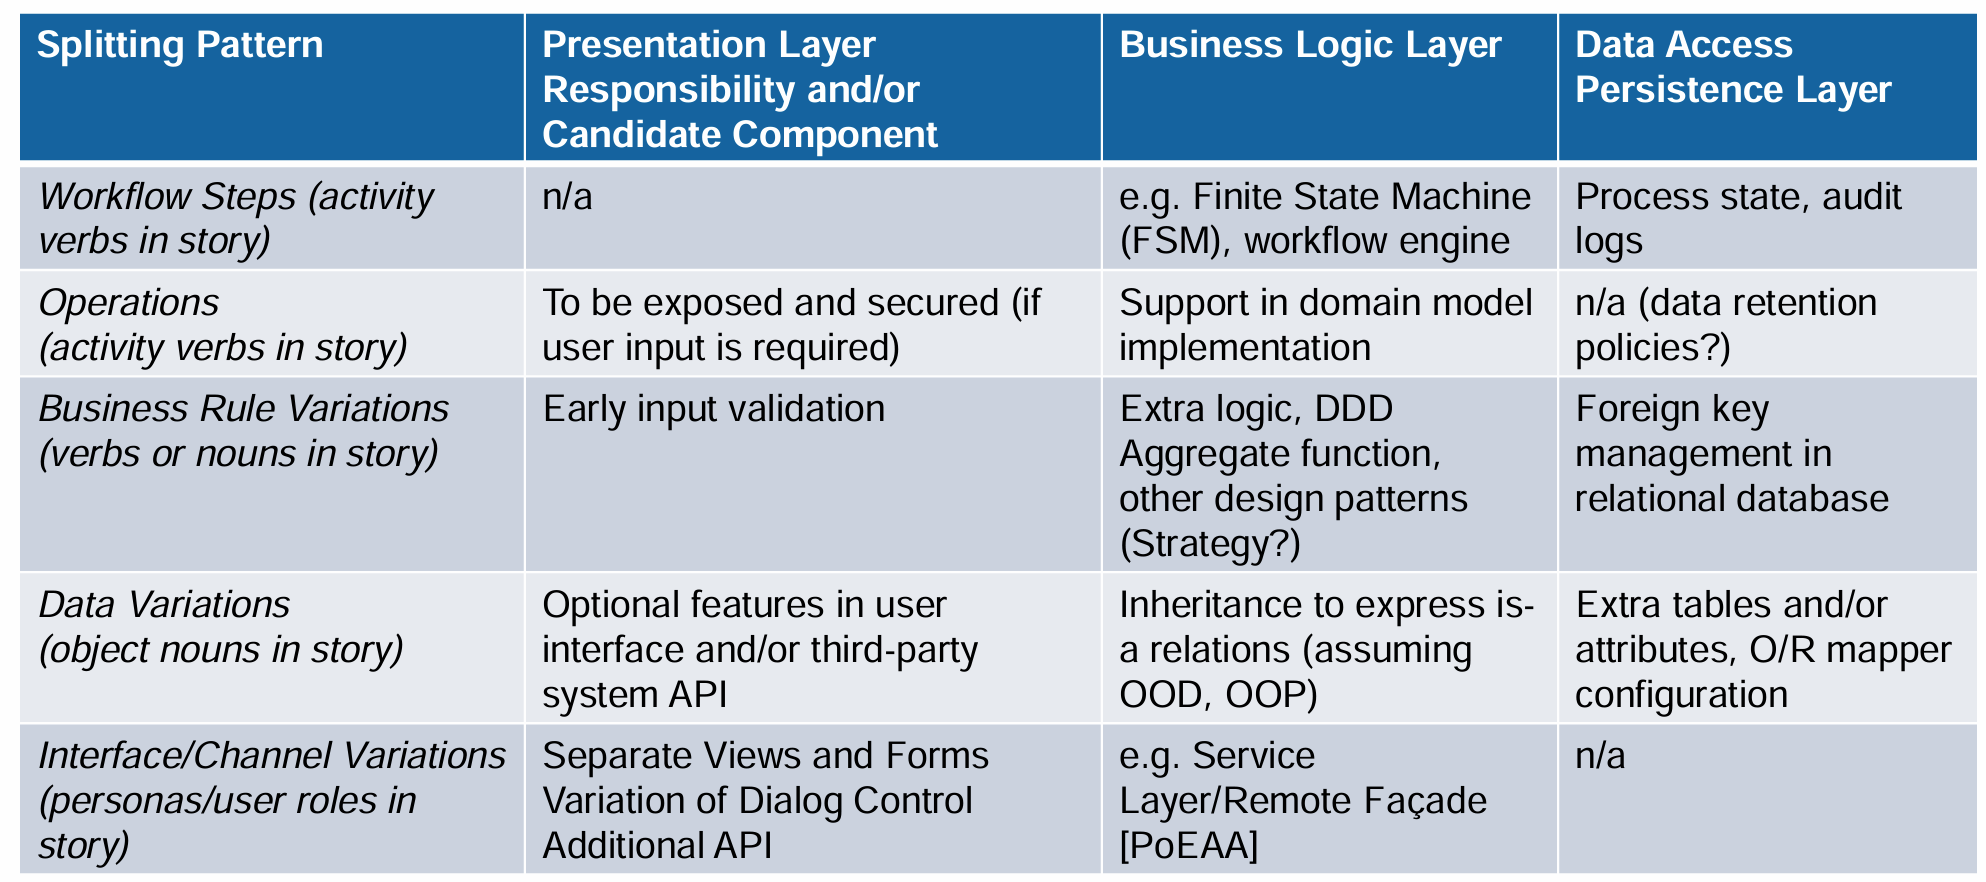
\includegraphics[width=1\linewidth]{Images/user-stories-components.png}
    \caption{User Stories for Components Example}
\end{figure}

\subsubsection{Identification}
A rule of thumb is to identify one candidate component per layer and
feature or entity without knowing too much about them.
OOAD and business modeling techniques can help with CI.
\begin{itemize}
    \item Partition by domain concepts (single responsibility principle)
    \item Partition by stakeholders or users (No reimplementations per user story (DRY!))
    \item Partition by product or data types (domain model entities)
    \item Add feature or component for locations and regions
    \item External interfaces to other systems
\end{itemize}

\section{Patterns of Enterprise Application Architecture (PoEAA)}

The PoEAA book(Fowler(2002)) only has one pattern called Domain Model to represent an object-oriented BLL,
and describes Transaction Script and Table Module as alternatives. 

The Business Logic Layer patterns in the PoEAA book are rather simplistic (which is somewhat surprising) and
superseded and refined by Domain-DrivenDesign (DDD).
%TODO

\section{Tactic Domain Driven Design (DDD)}
In DDD the domain model is put in the center. It emphasizes the need for
modeling and communication in a ubiquitous language, the domain model.
Tactic DDD focuses on business logic in layered architecture models.
It does so by decomposing the domain model pattern from Martin Fowler.
It contains patterns for common roles.

In \textbf{Strategic DDD} the emphazis lies in enterprise architecture and
portfolio management. Boundaries are very important in a macroscopic view.

\begin{figure}[H]
    \centering
    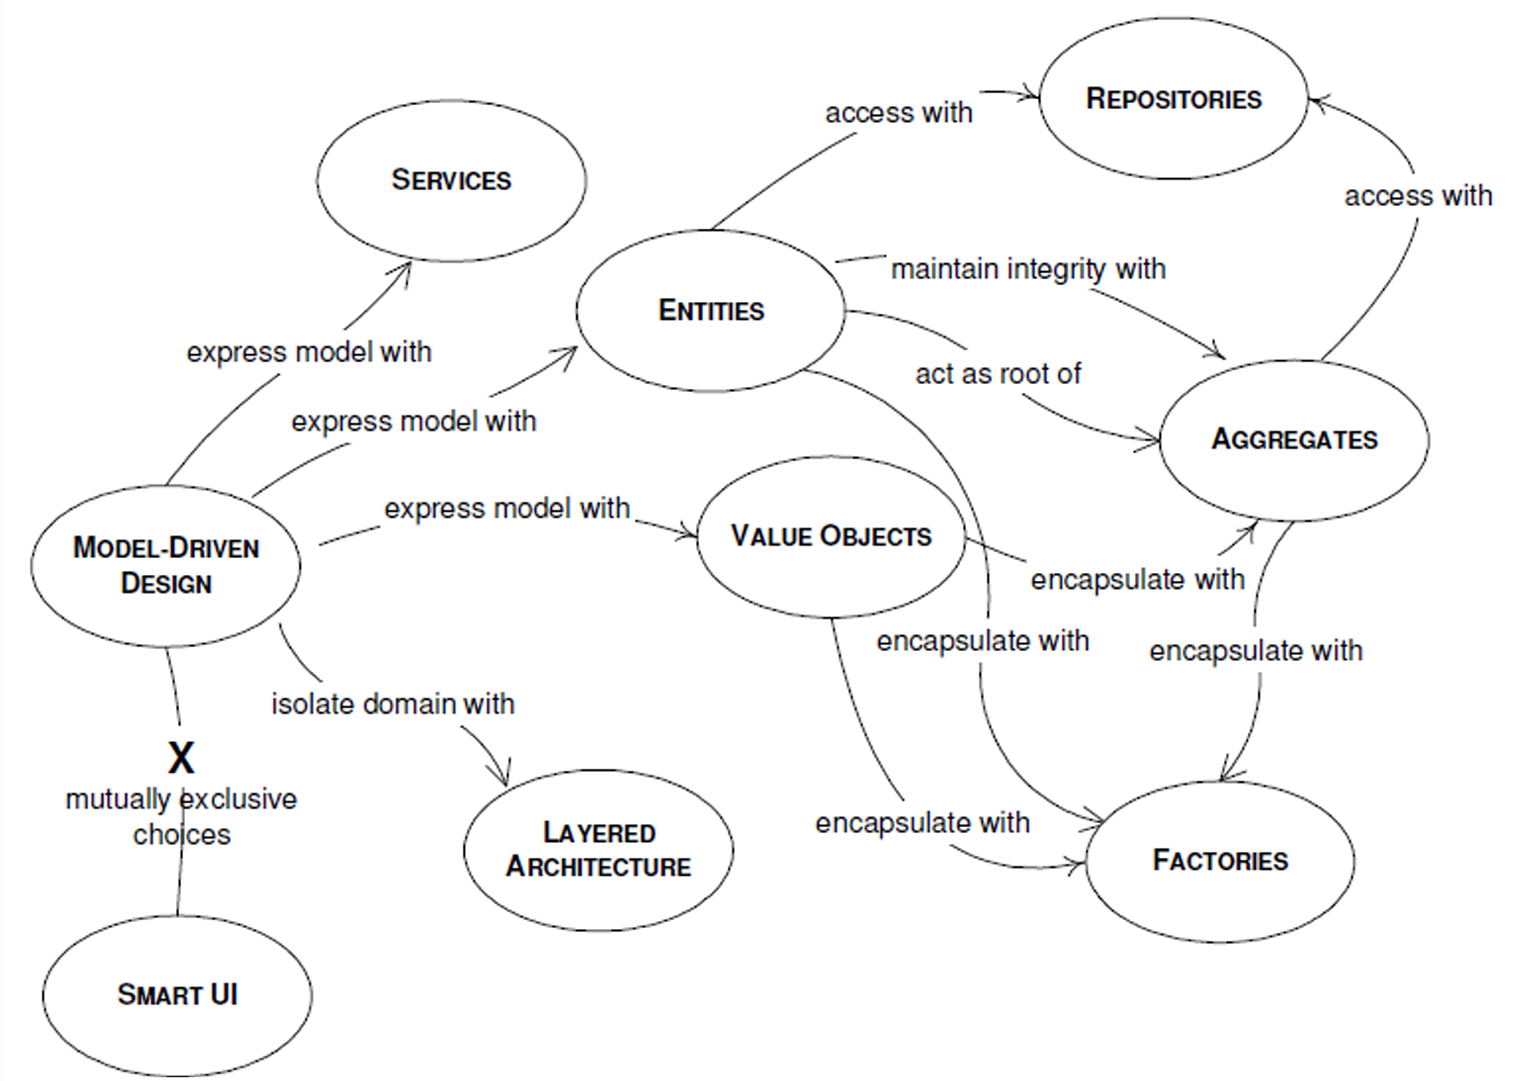
\includegraphics[width=1\linewidth]{Images/patternmap-tactic-ddd.png}
    \caption{Tactic DDD - Pattern Map}
\end{figure}

\subsection{DDD and Logical Layers}
Layered Architecture pattern in DDD is not identical to PoEAA schema, but
it can be mapped in an easy way:
\begin{figure}[H]
    \centering
    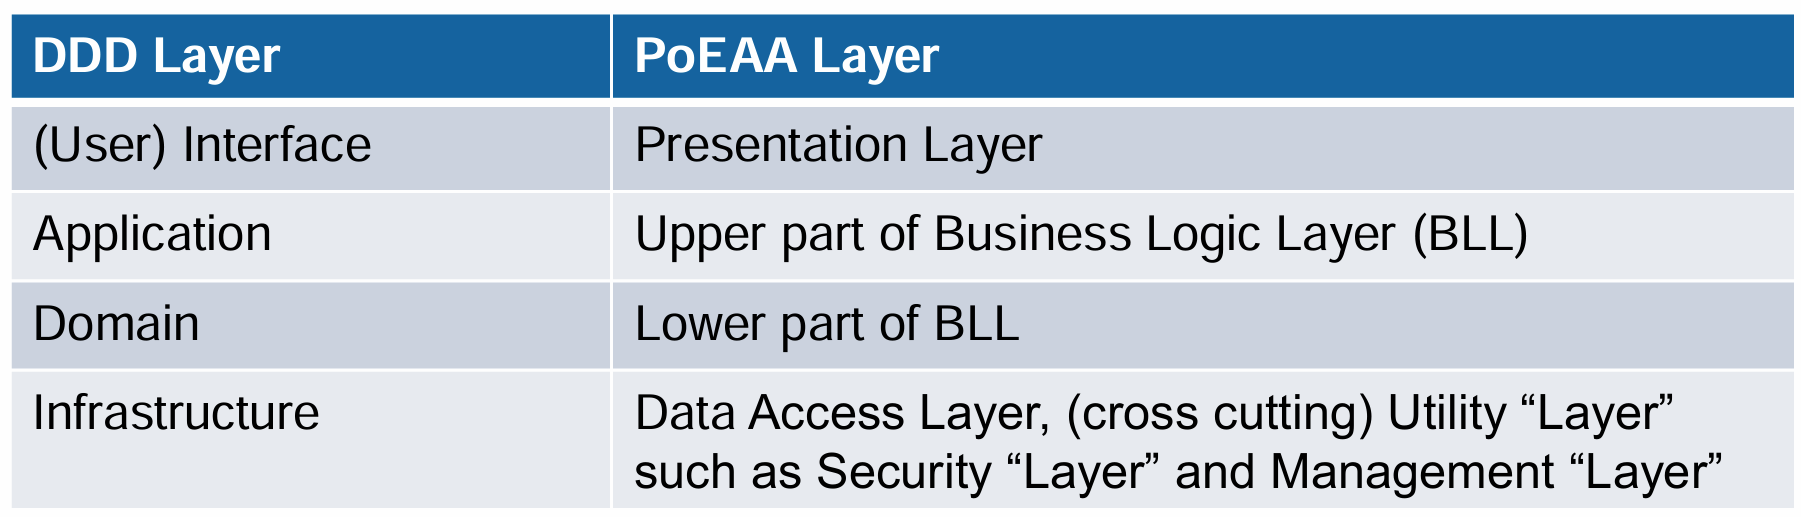
\includegraphics[width=1\linewidth]{Images/ddd-logical-layers.png}
    \caption{DDD and Logical Layers}
\end{figure}
The instances of tactic DDD primarily lives in the domain layer.

\begin{figure}[H]
    \centering
    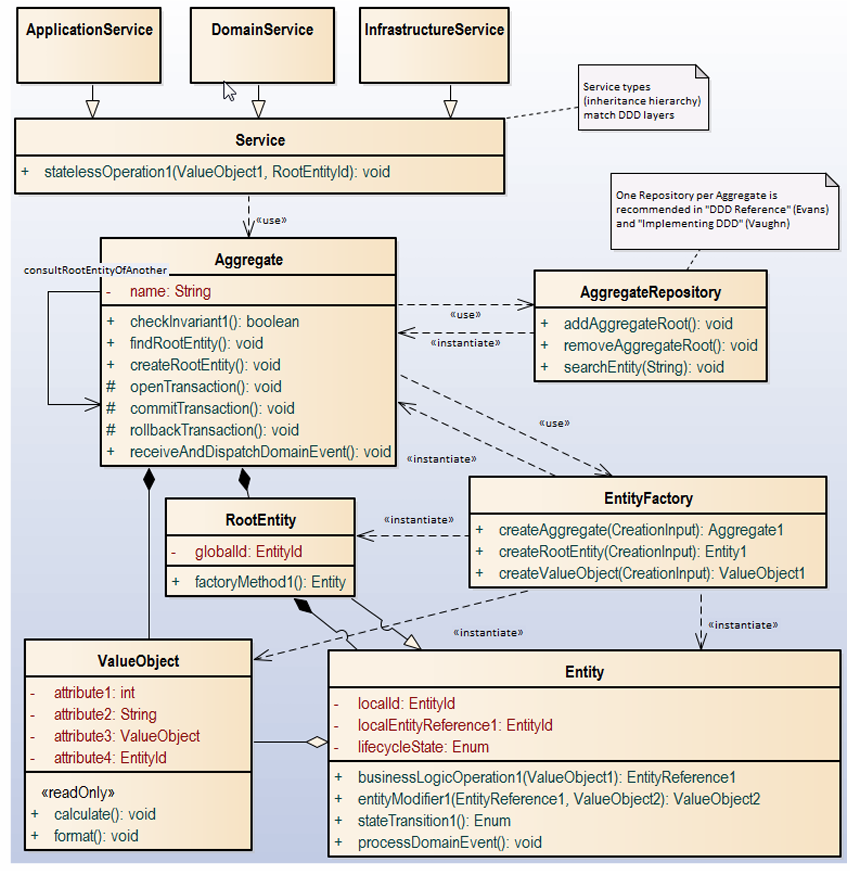
\includegraphics[width=1\linewidth]{Images/ddd-meta-model.png}
    \caption{DDD Domain Meta model}
\end{figure}

\subsection{Entity}
Entity is an object that has an identifier and a lifecycle.
It can change states and can be distringuished by its identity
and therefore is not defined by its attributes.

\subsection{Value}
The value object has no identifier and is immutable.
Hence it has no state and is soely defined by its attribute.
All operations on the value object must be side effect free.

\subsection{Aggregate}
An aggregate is a collection (or graph) of entities and value objects.
It is the smallest unit with functional consistency while enforcing invariants.
All objects of an aggregate are persisted toghether, this means
the transaction boundary is around the collection.
The aggregates has a root entity as external interface and entry point.
External object should only reference the root entity.
Aggregates are responsible for business rule enforcement accross entities.

\begin{figure}[H]
    \centering
    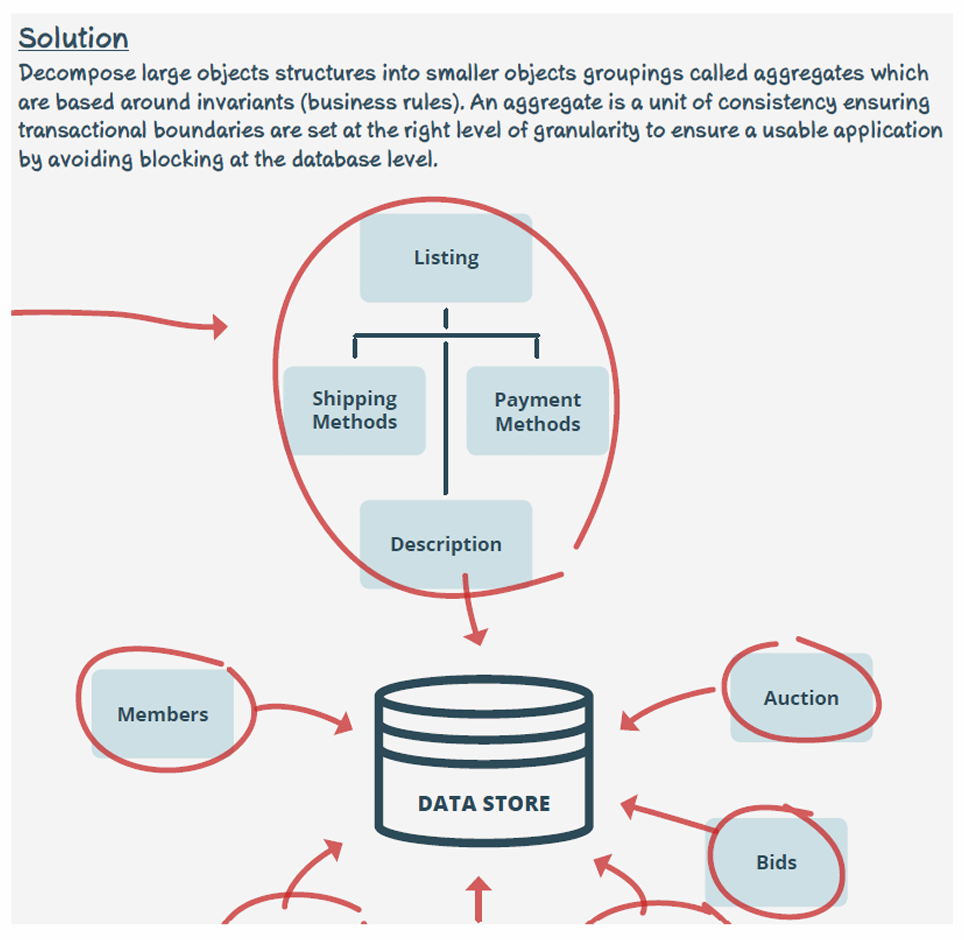
\includegraphics[width=1\linewidth]{Images/aggregate.png}
    \caption{Aggregate}
\end{figure}

\begin{figure}[H]
    \centering
    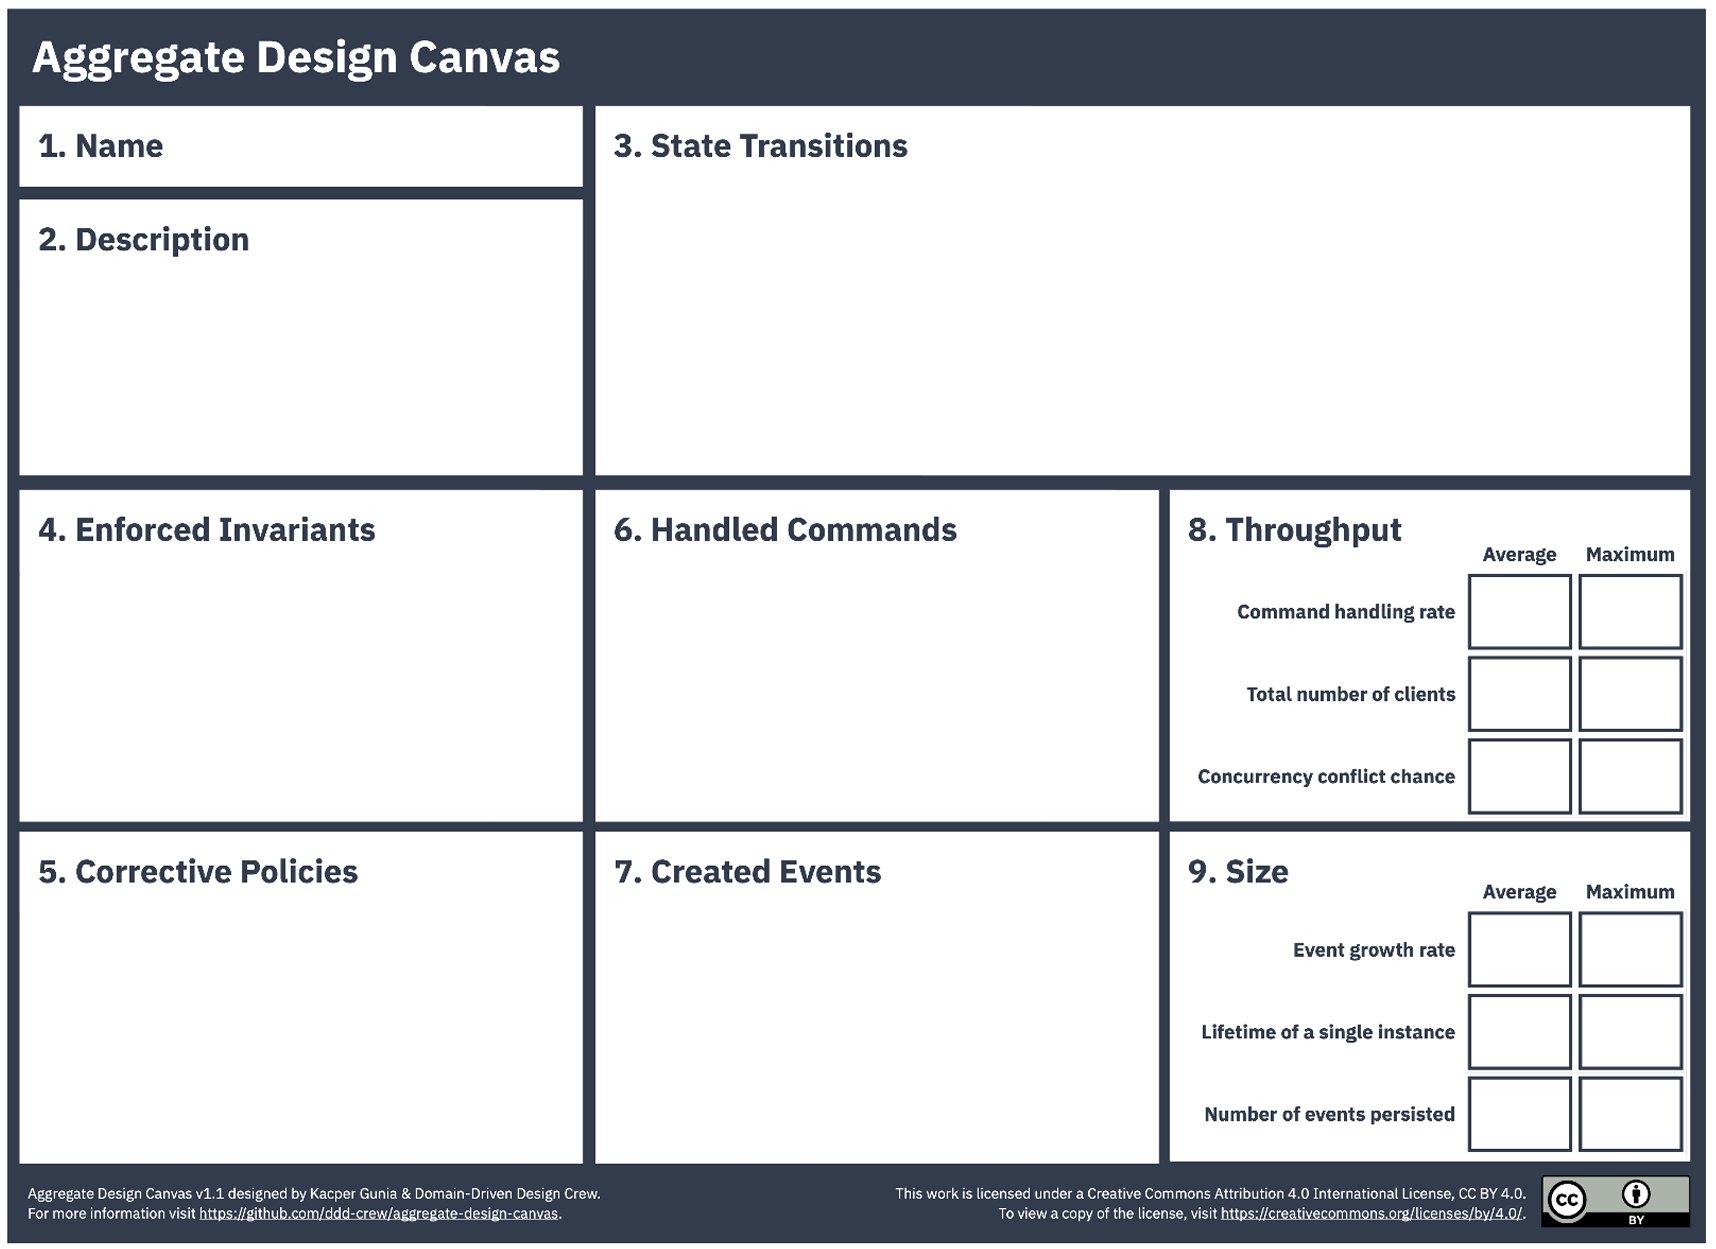
\includegraphics[width=1\linewidth]{Images/aggregate-design-canvas.png}
    \caption{Aggregate Design Canvas}
\end{figure}

\subsection{Bussiness Rule and Invariants}
Business rule has (at least) two meanings:
\begin{enumerate}
    \item Executable part of the business logic that is not expressed as sequence of statements, but declaratively
    \item A statement or condigtion about the domain model, its elements and their relationship that always has to be true (invariant),
    to preserve data consistency and ensure accuracy of processing
\end{enumerate}

Examples of Invariants:
\begin{itemize}
    \item Physical containment relationship. (No order without an existing customer)
    \item Number calculations/value ranges (Total sum must not exceed value Y)
    \item Accounting and non-repudiation (All calls are billed)
\end{itemize}

\subsection{Service}
A service exposes domain logic that crosses aggregate boundaries.
Domain logic that cannot be assigned to a domain object naturally.
The service is itself stateless and has several variants by sublayer:
\begin{itemize}
    \item Domain services (core logic)
    \item Application services (not in domain model)
    \item Utility services
\end{itemize}

\subsection{Event}
An event is a representation of something that happened in the domain.
Model activity is represented in the domain as a series of domain events.
The events themselves are immutable. A domain event is always something
that happened in the past, and since we cannot change the past, it is immutable.
Events may be exchanged between aggregates.

\subsection{Repository}
The repository is an entity that handles persistence of the aggregates.
There may be one repository per aggregate and it interacts with the root entity.
Repositories themselves do not contain business logic and only the interface
belongs to the core domain model. This makes the implementation replaceable.

\subsection{Best-Practices}
\begin{itemize}
    \item Use asynchronous communication between aggregates
    \item Give enforcement responsibilities to root entity, possibly supported by designated framework mechanisms
    \item Keep one aggregate on one server, allow different aggregates to be distributed among hardware
    \item Use the same boundaries for transactions and distribution
    \item Model true invariants in consistency boundaries
    \item Design small aggregates
    \item Reference other aggregates by identity
    \item Use eventual consistency outside the boundary
\end{itemize}

\subsection{CRC Cards}
The CRC card is a notation that is well suited for component modeling, 
complementing C4. CRC stands for Components, Responsibilities, Collaborators.
CRC must be expressive, but also easy to understand.

\begin{figure}[H]
    \centering
    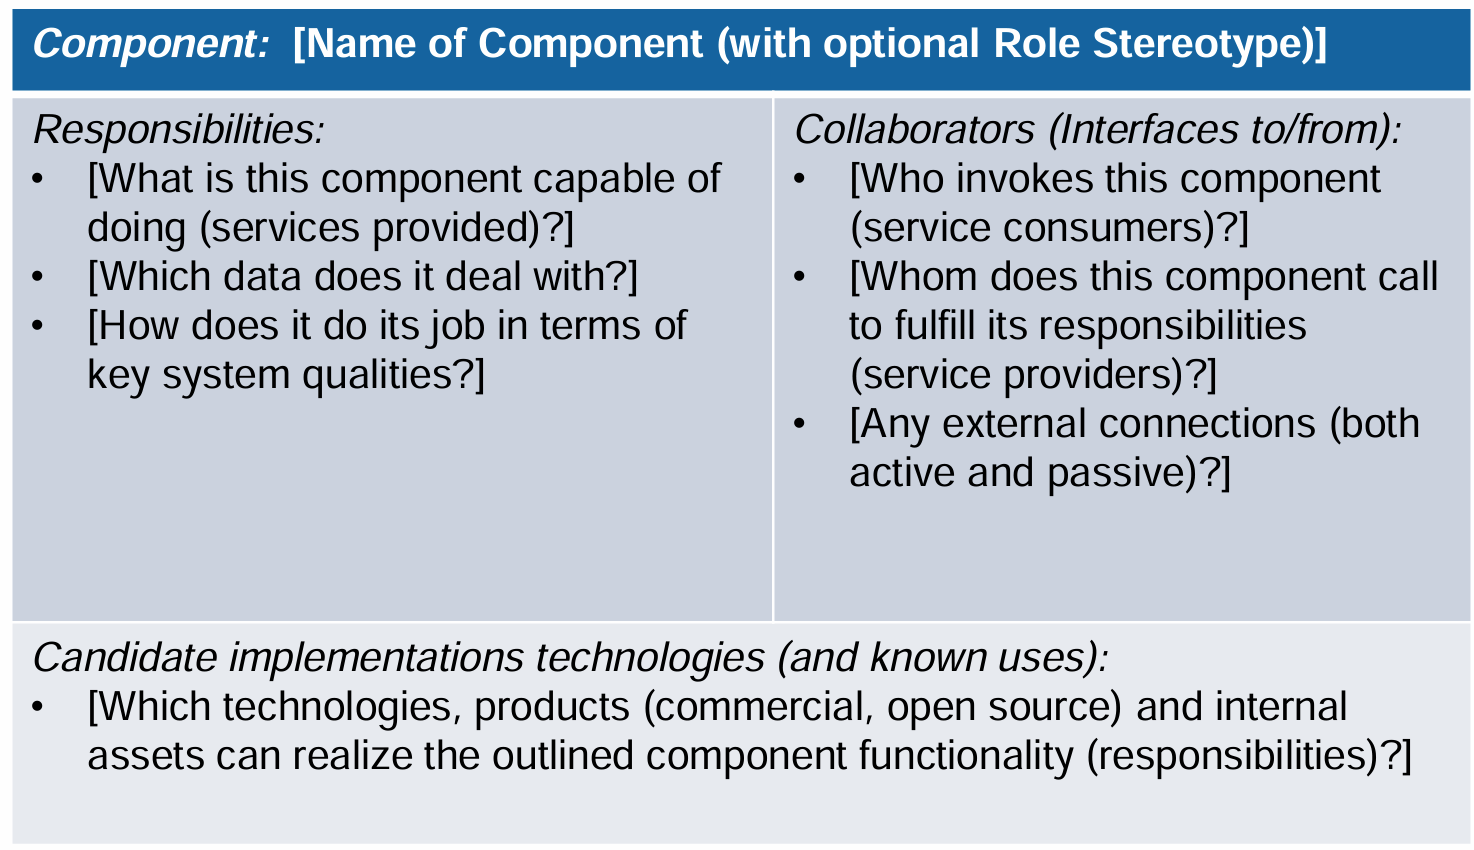
\includegraphics[width=1\linewidth]{Images/crc-card.png}
    \caption{CRC Card Template}
\end{figure}

\subsection{OOA to Tactic DDD}
\begin{enumerate}
    \item Distinguish Entities (stateful) and value objects (stateless). Put non-OO code in services
    \item Group output of step 1 into aggregates (storage units). Let aggregates communicate state changes via domain events.
    \item Add a repository for each aggregate. One may also add factories.
\end{enumerate}

\section{Strategic DDD}
Strategic Domain Driven Design is concerned with designing the domain
model inside a bounded context.

\subsection{Bounded Context (BC)}
Bounded Contexts are descriptions of a boundary within which a particular model
is defined and applicable.
Bounded contexts implement parts of one or multiple subdomains.
Subdomains are specific problem spaces as a result of object oriented analysis.
Bounded context are in the solution space and are a result of object oriented design.
Four advantages of using model partitioning and context boundaries:
\begin{itemize}
    \item Same term, different meaning (homonym)
    \item Same concept, different different use (polyseme)
    \item External system differences (heterogeneity)
    \item Scaling up the organization (multiple teams)
\end{itemize}

\begin{figure}[H]
    \centering
    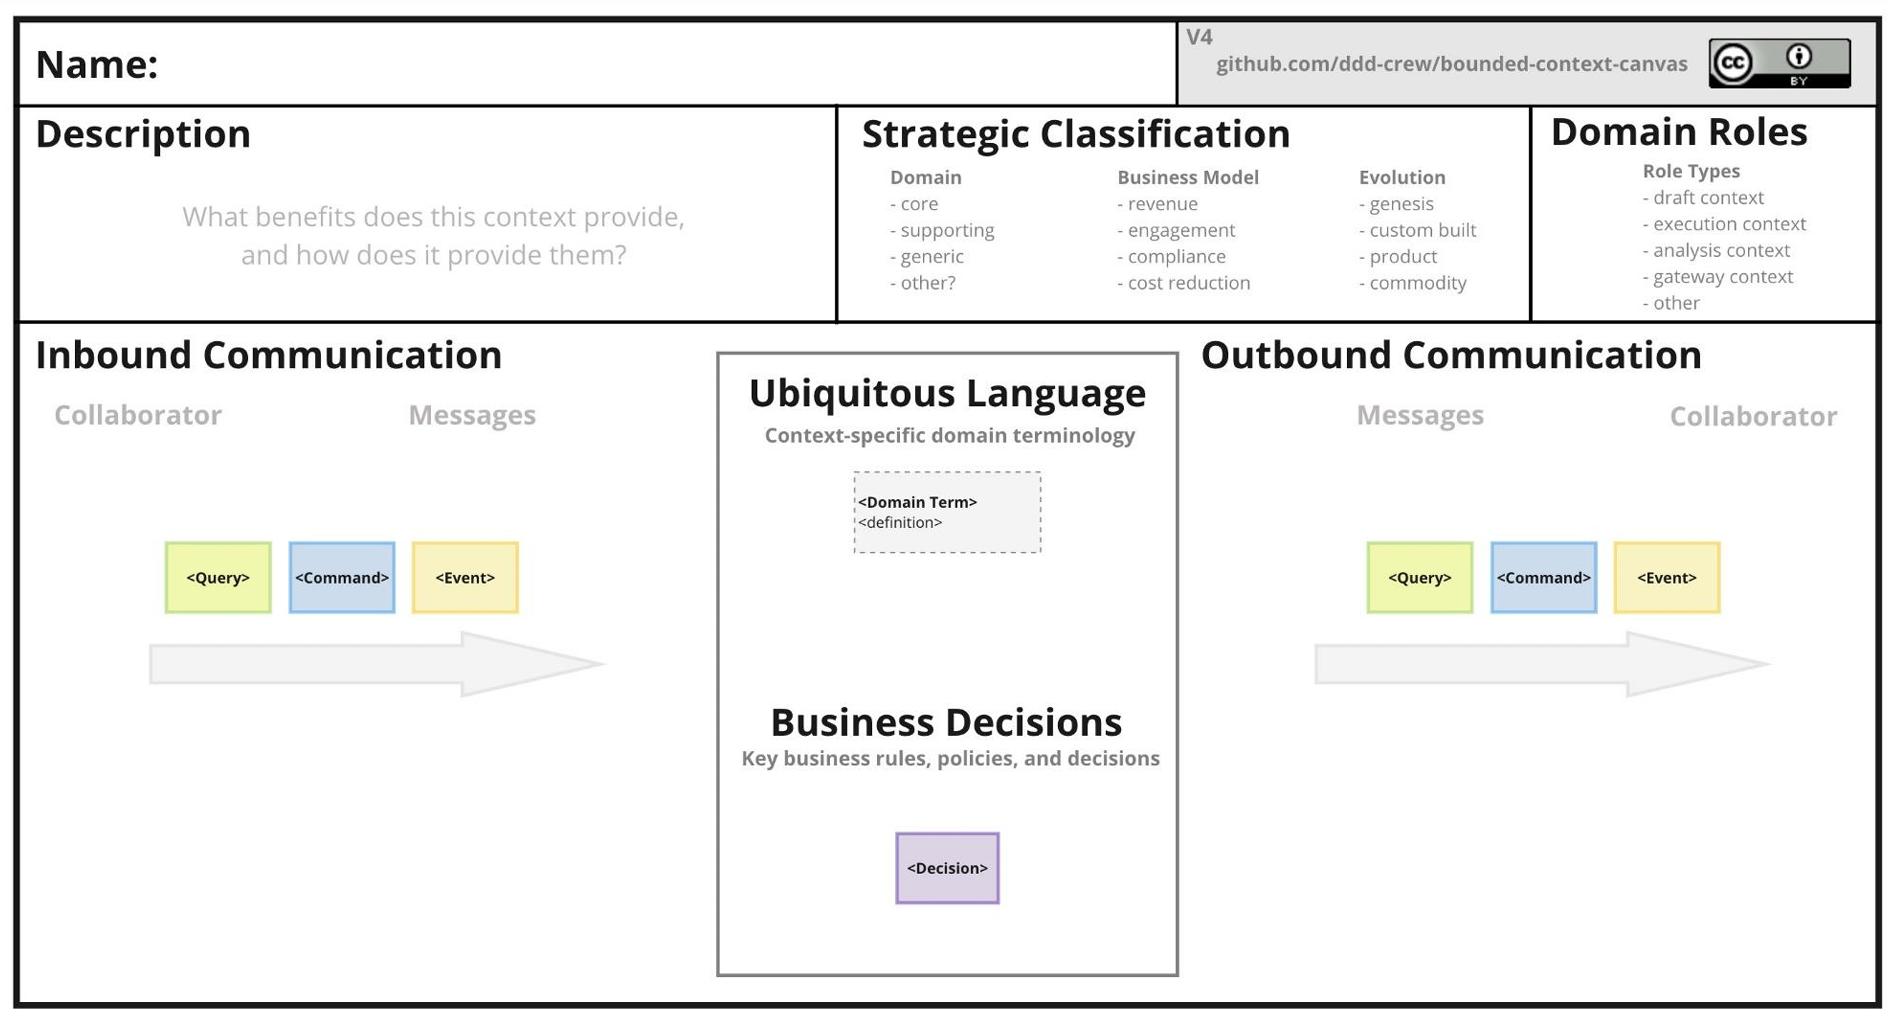
\includegraphics[width=1\linewidth]{Images/bounded-context-canvas.png}
    \caption{Bounded Context Canvas}
\end{figure}

\begin{figure}[H]
    \centering
    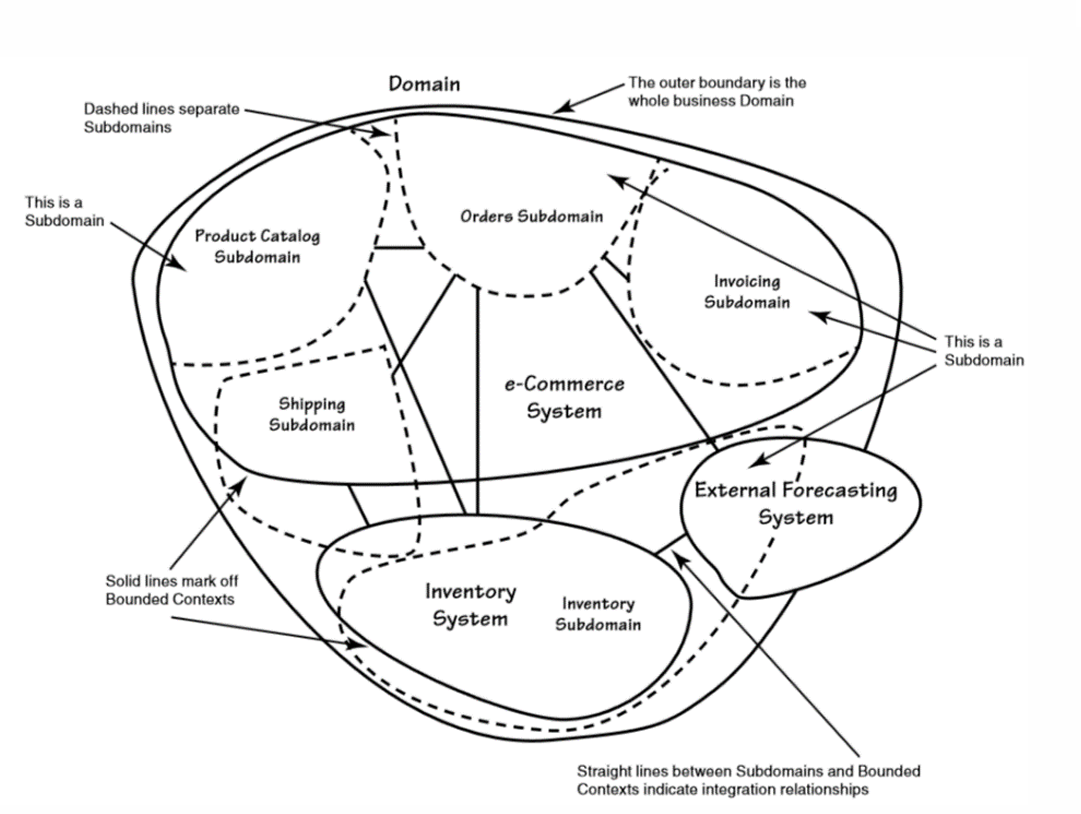
\includegraphics[width=1\linewidth]{Images/subdomains-bounded-context.png}
    \caption{Subdomains vs Bounded Context}
\end{figure}

\begin{figure}[H]
    \centering
    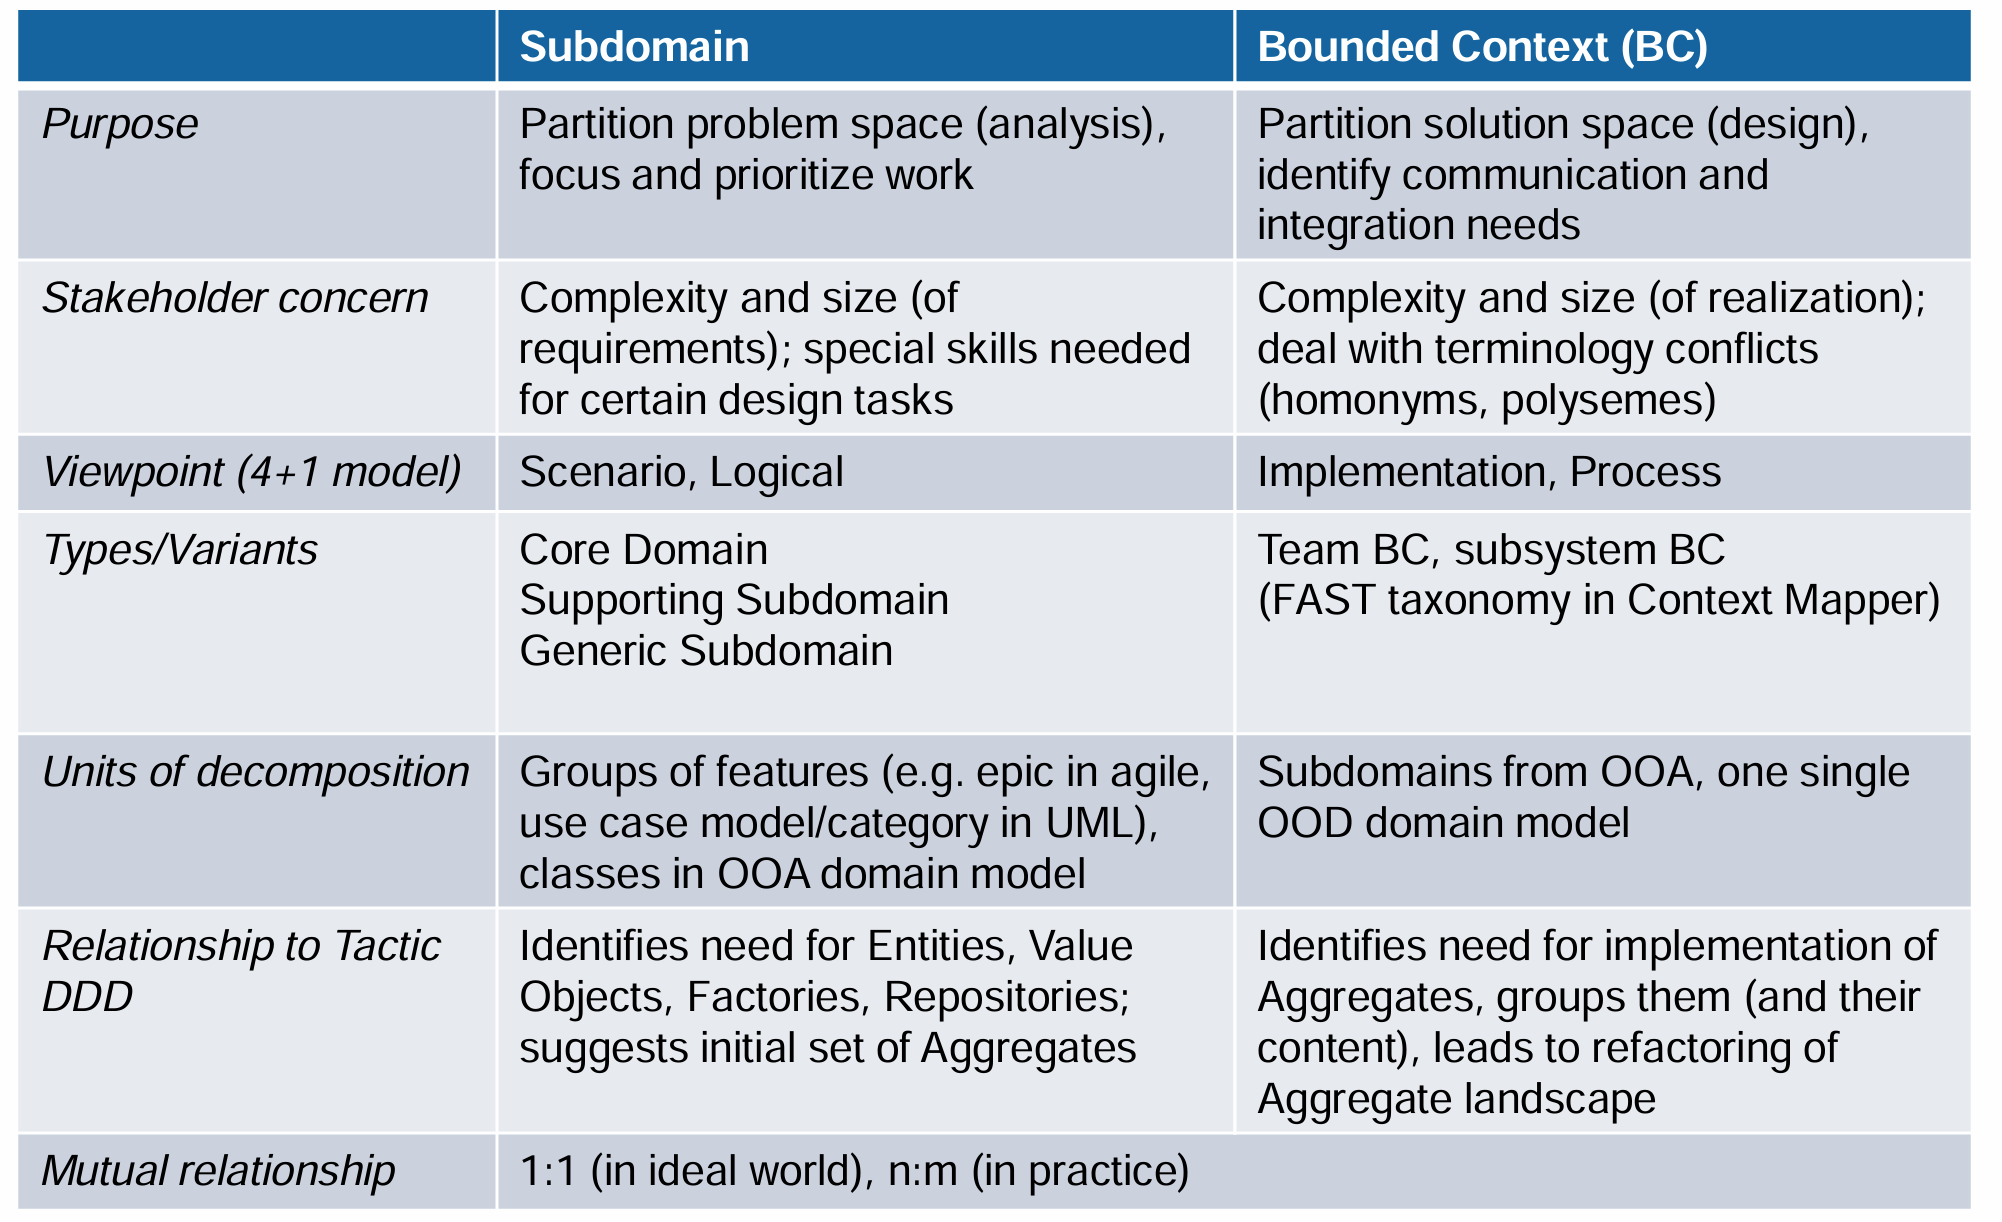
\includegraphics[width=1\linewidth]{Images/subdomain-vs-bc.png}
    \caption{Subdomains vs Bounded Context Comparison}
\end{figure}

\section{AB CHAPTER??? 5-6-7??}

%chapter 12-13
\section{Service Orientation}
\subsection{Service Layer Pattern}
\subsection{Service Oriented Architecture (SOA)}

\subsection{Hate-OAS}
\begin{figure}[H]
    \centering
    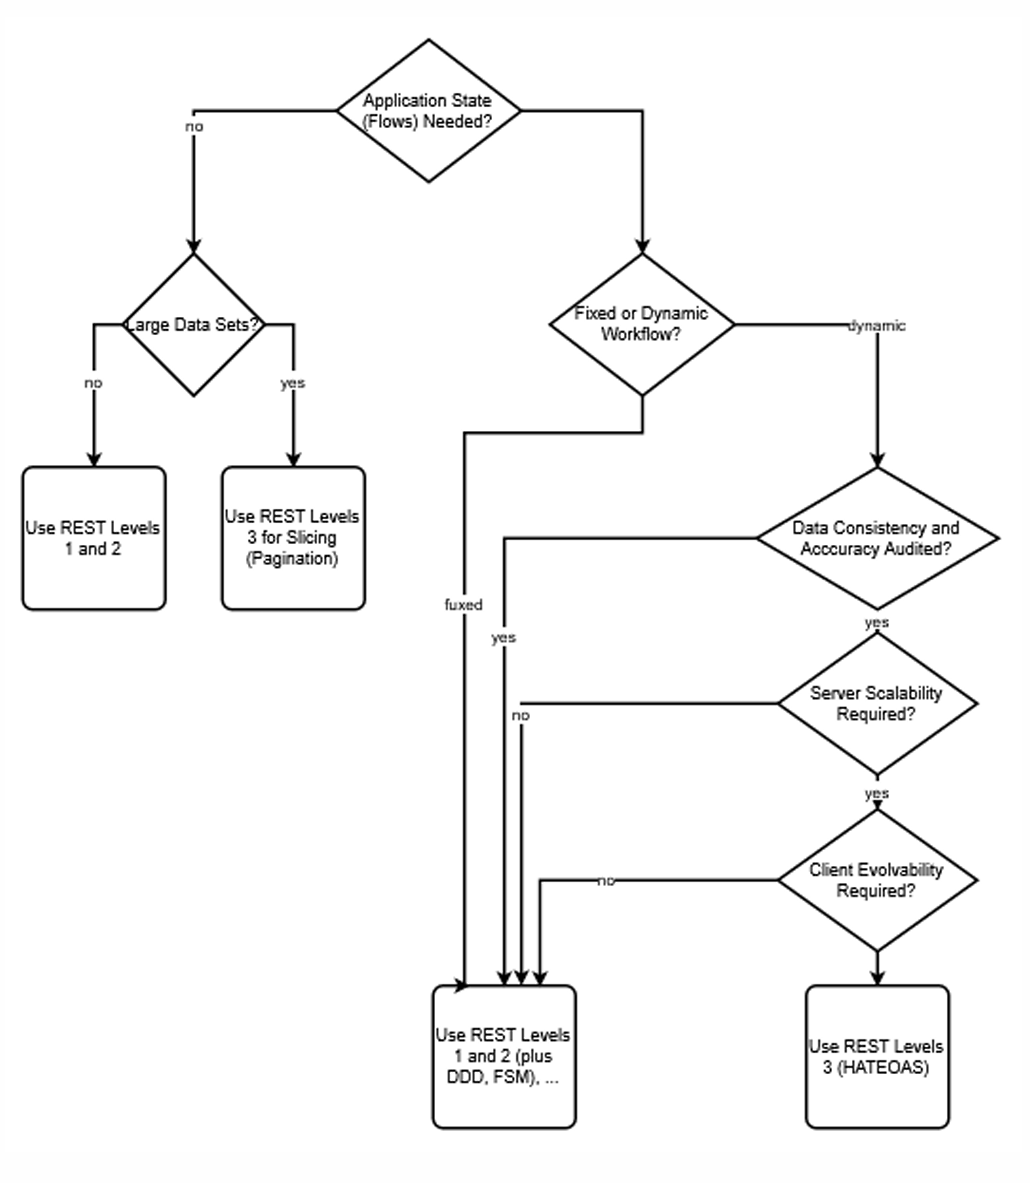
\includegraphics[width=0.5\linewidth]{Images/hate-oas-dectree.png}
    \caption{Decision Tree for Hate-OAS}
\end{figure}

WHO IS IN CHARGE OF STATE TBD

\subsection{Microservices and SOA}

Many Enterprise Integration Patterns (EIP) are usable in SOA or in Microservice Design.
E.g some patterns that can be applied:
\begin{description}
    \item[Messaging Gateway] Interoperability between Messaging Systems
    \item[Message Bus] See EIP
    \item[Service Activator] Kind of a middleware see in EIP
    \item[Process Manager] Pattern from Message Routing. Communication of queues are coordinated over the manager (orchestrator)
    There are many available applications for this (EAI, Message Broker)
\end{description}

\defn{Microservices Architecture by Fowler}{
    The microservice architectural style is an \textbf{approach to developing a single application 
    as a suite of small services}, each running in its \textbf{own process} and communicating with 
    \textbf{lightweight mechanisms}, often an\textbf{HTTP resource API}
}
These services are built around business 
capabilities and independently deployable by fully automated deployment machinery.
There is a bare minimum of centralized management of these services, which may be written in
different programming languages and use different data storage technologies.

\defn{Principles (Newman)}{
    \begin{itemize}
        \item Model around business concepts (Bounded Context from DDD)
        \item Adopt a
    \end{itemize}
}

Some of the advantages can be the following:
\begin{itemize}
    \item High Velocity due to reduced communication
    \item Some technological independence (e.g. frameworks and languages)
    \item Improved maintainability (in theory)
    \begin{enumerate}
        \item Can be replaced easily
        \item Architecture might be less prone to erosion, because boundaries are harder to overcome
    \end{enumerate}
    \item Suited for cloud deployment due to distributed nature, isolated state and other cloud properties.
    \item Scalability (individually)
    \item Failure safety (due to individual services)
\end{itemize}
But SOA should not be used blindly, since it also comes with disadvantages:
\begin{itemize}
    \item Increases complexity e.g. due to more components or coordination
    \item Overhead in communication
    \item More platform requirements
    \item More (...)
\end{itemize}

\subsection{Service Contracts}

\section{Other Tools and Methods}
\section{C4 Model}
\defn{C4 Model}{
The C4 model is a software architecture visualization model based on a set of hierarchical abstractions: software systems, containers, components, and code. It uses corresponding hierarchical diagrams—System Context, Container, Component, and Code—to describe these abstractions. The model is intentionally notation-independent and tooling-independent, focusing on clarity and adaptability rather than imposing specific methodologies or tools.
}
C4 model as a "light" alternative to UML. 
\begin{enumerate}
    \item First level of design (solution strategy): containers
    \item Second level of design (refinement): components
    \item Third level of design coded, not diagrammed (construction)
\end{enumerate}

Context matters (the first C in C4), System Context Diagram (SCD) also present in other software engineering and architecture design methods

\begin{figure}[H]
    \centering
    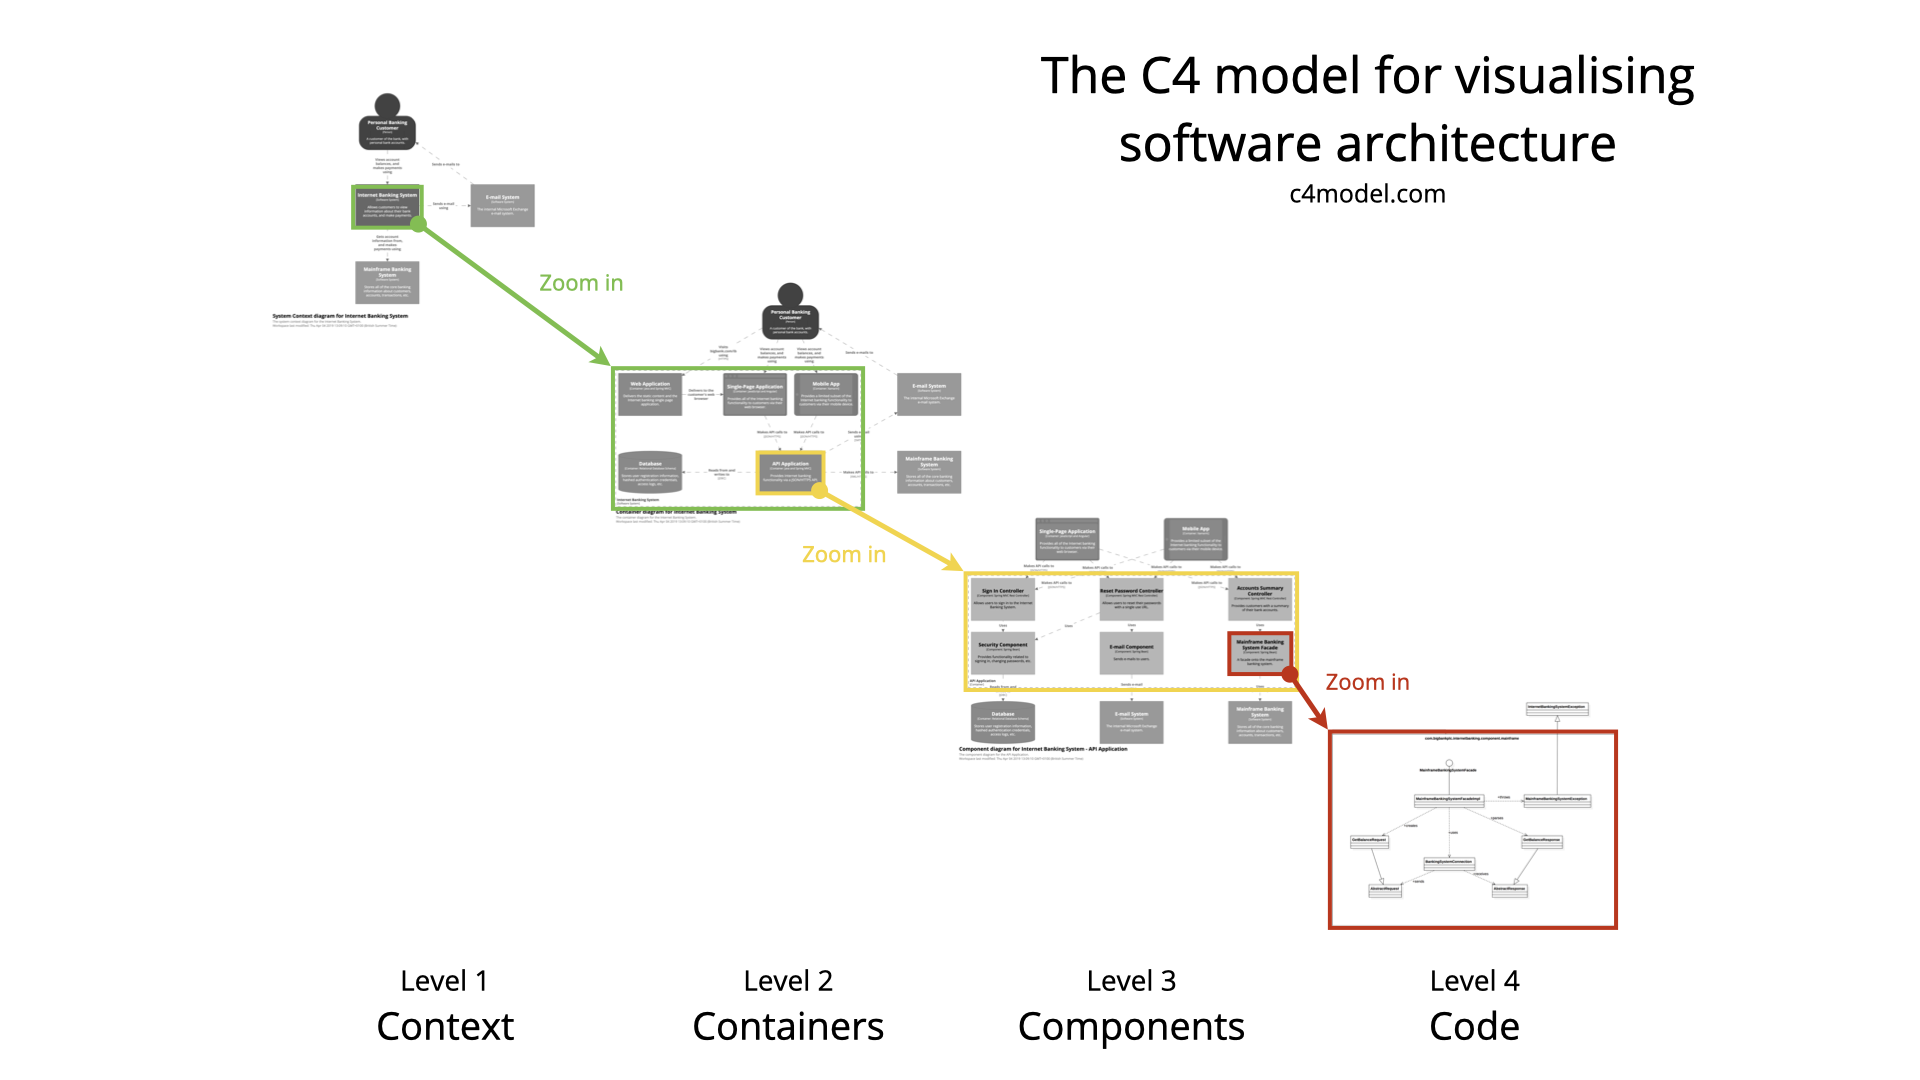
\includegraphics[]{Images/c4-overview.png}
    \caption{C4 Model Overview}
\end{figure}
\href{https://c4model.com/}{Link to C4 Model Home Page}

%\newpage
%\section{Onion}
%\begin{figure}[H]
%    \centering
%    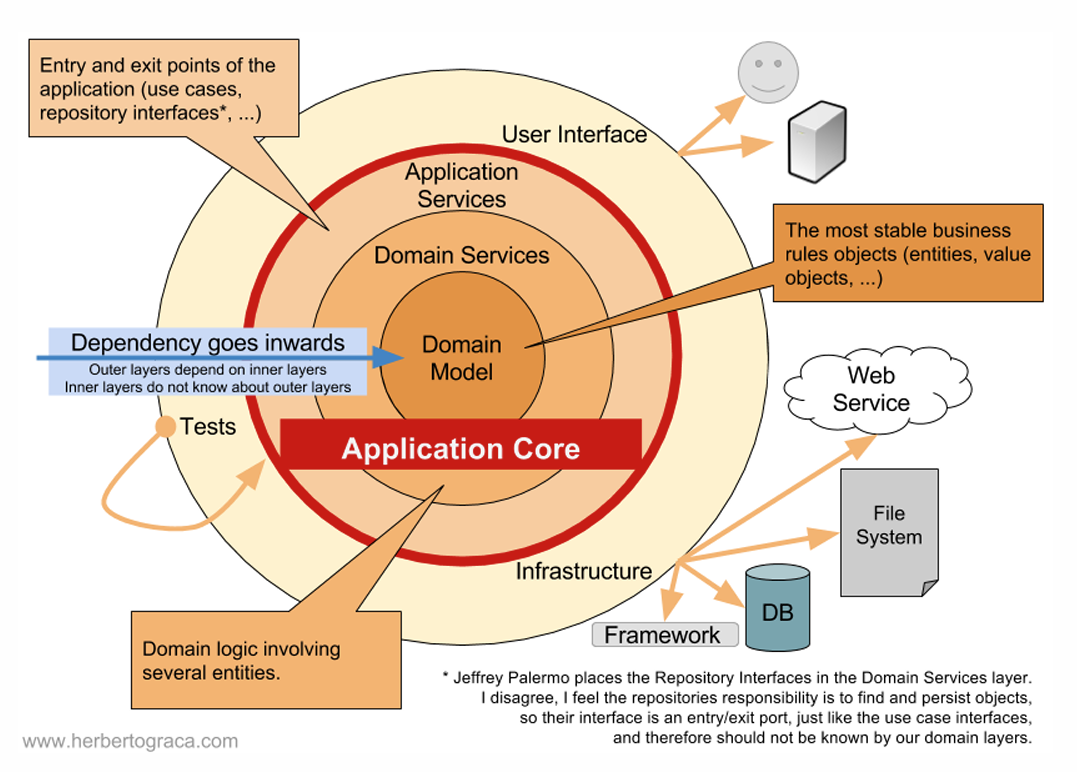
\includegraphics{Images/onion.png}
%    \caption{Onion Architecture}
%\end{figure}

\newpage

\subsection{Story Splitting Flowchart}
A story that is too large for a sprint must be broken down
to meet the INVEST properties of user stories.
\begin{figure}[H]
    \centering
    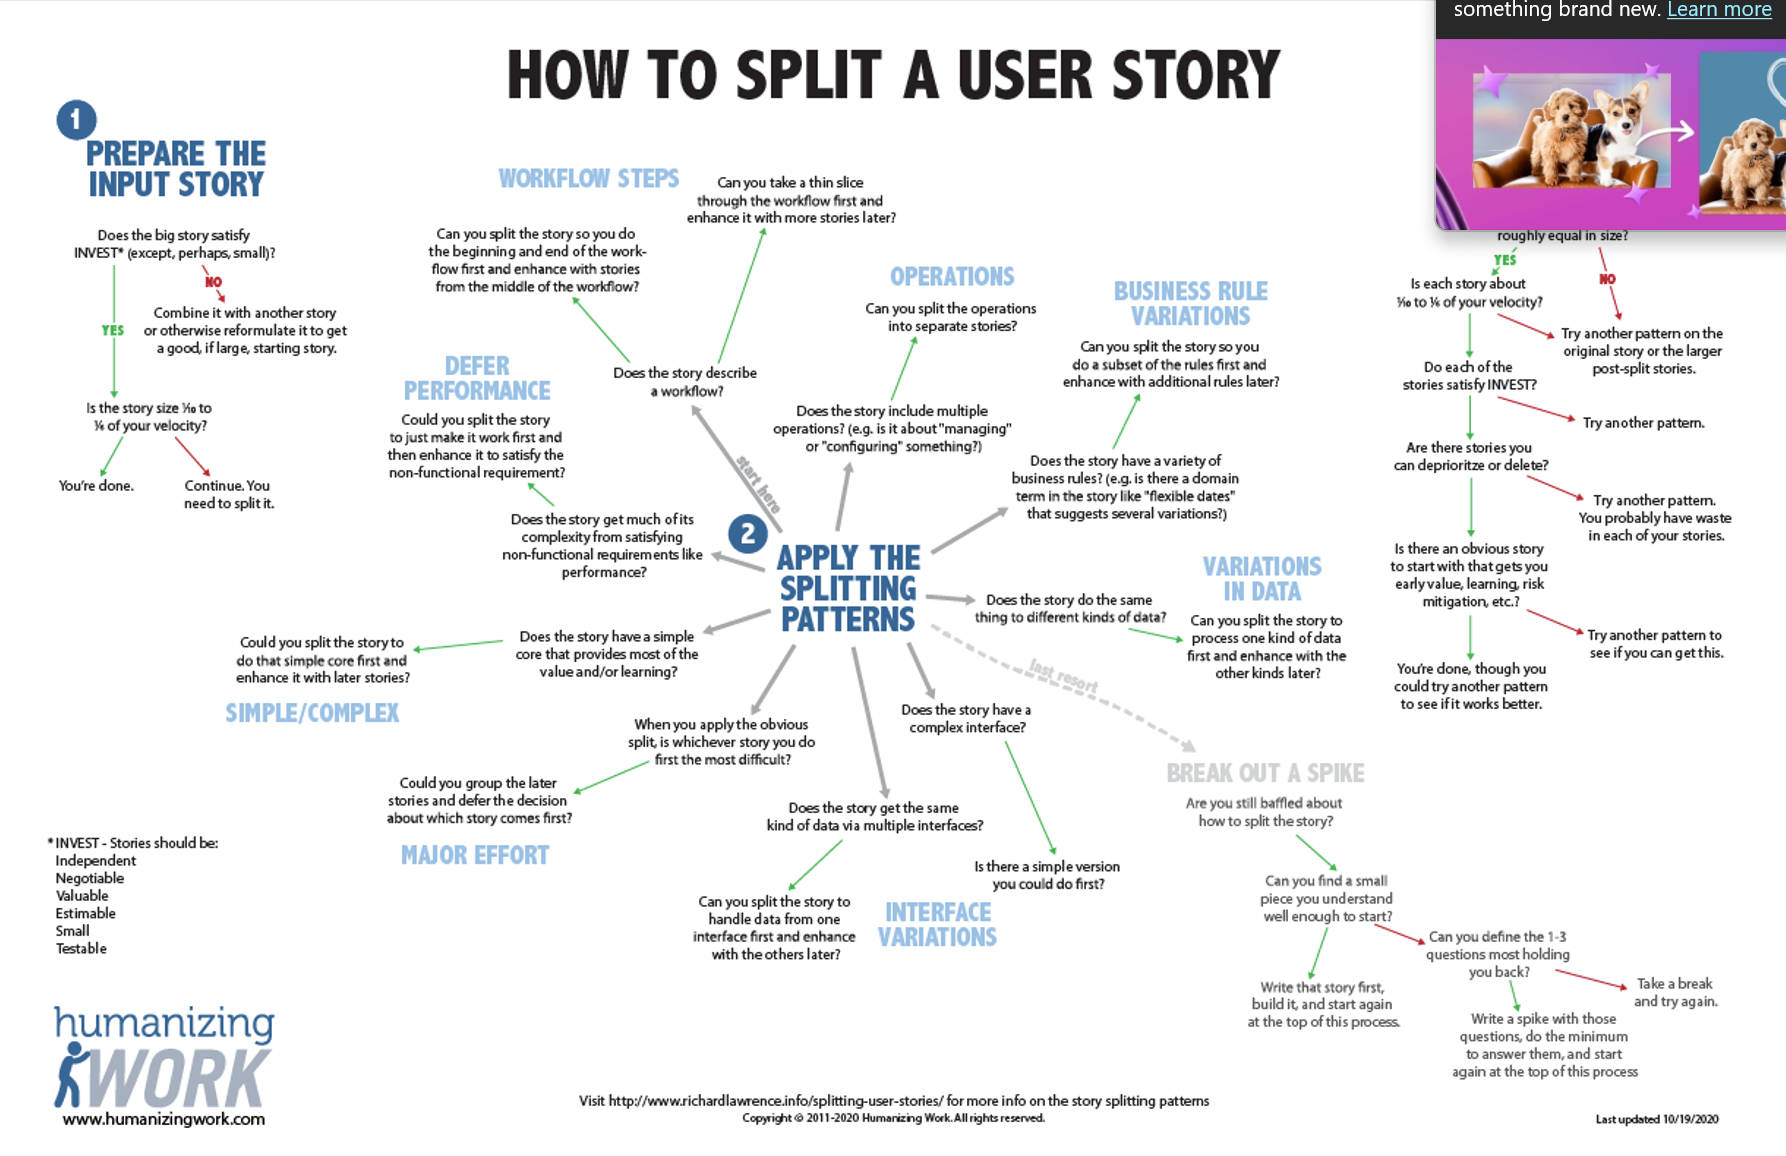
\includegraphics[angle=90,height=1\textwidth]{Images/storysplitting.png}
    \caption{Story Splitting Flowchart}
\end{figure}
\newpage

\begin{figure}[H]
    \centering
    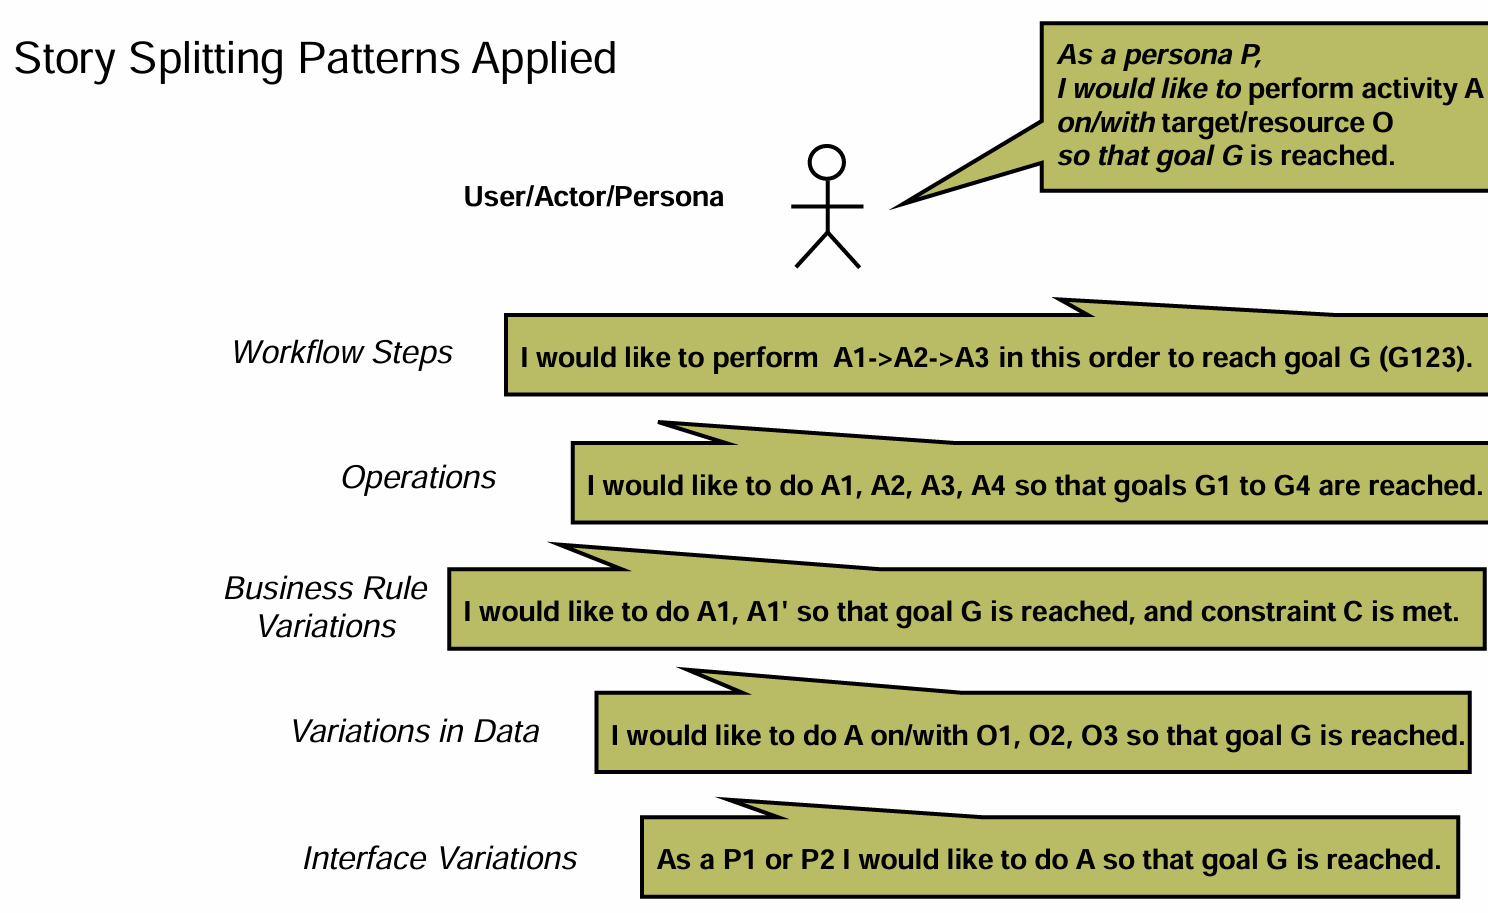
\includegraphics{Images/appliedstorysplitting.png}
    \caption{Story Splitting Example}
\end{figure}

\begin{table}
    \centering
    \begin{tabular}{|c|c|c|c|} \hline 
        Splitting Pattern&  Pres. Layer Responsibility &  Business Logic& Data Access Layer\\ \hline 
        Workflow Steps&  &  & \\ \hline 
        Operations&  &  & \\ \hline 
        Business Rule&  &  & \\ \hline 
        Data Variations&  &  & \\ \hline 
        Interface Variations& & &\\ \hline
    \end{tabular}
    \caption{Story Splitting Example Table}
    \label{tab:storysplitex}
\end{table}

\end{document}
